\documentclass[12pt, a4paper]{extreport}
\usepackage[margin=1.5cm]{geometry}
\usepackage{amsmath}
\usepackage{graphicx}
\usepackage{caption}
\usepackage{subcaption}
\usepackage{float}
\usepackage{wasysym}
\usepackage[procnames]{listings}
\usepackage{color}

\definecolor{keywords}{RGB}{255,0,90}
\definecolor{comments}{RGB}{0,0,113}
\definecolor{red}{RGB}{160,0,0}
\definecolor{green}{RGB}{0,150,0}
 
\lstset{language=Python, 
        basicstyle=\ttfamily\small, 
        keywordstyle=\color{keywords},
        commentstyle=\color{comments},
        stringstyle=\color{red},
        showstringspaces=false,
        identifierstyle=\color{green},
        procnamekeys={def,class}}
% ===============================================================
\begin{document}
\begin{flushleft}
{\large\textbf{1) Construct the phase portrait for Problem 2.1g of Nayfeh and Mook.}}
\end{flushleft}

The potential function for the following equation can be constructed by integrating the force function, $f(x)$. The equation of motion is defined as
%
\begin{equation}\label{eq:equationOfMotion}
	\ddot{u} + u - \frac{\lambda}{a - u} = 0
\end{equation}
%
The force function in above equation is
%
\begin{equation}
	f(u) = u - \frac{\lambda}{a - u}
\end{equation}
%
Therefore, the potential function can be calculated as:
%
\begin{subequations}
\begin{align*}
	F(u) &= \int f(u) du \\
		&= \int u - \frac{\lambda}{a - u} = \frac{u^2}{2} + \lambda \ln \left( |a - u| \right)
\end{align*}
\end{subequations}
%
Therefore, the potential function can be written as:
%
\begin{equation}
	F(u) = \frac{1}{2}u^2 + \lambda \ln \left( |a - u| \right)
\end{equation}
%
The mechanical energy consists of potential and kinetic energy. This can be written as:
%
\begin{equation}\label{eq:mechanicalEnergy}
	E(u) = \frac{1}{2} \dot{u}^2 + \frac{1}{2}u^2 + \lambda \ln \left( |a - u| \right)
\end{equation}
%
Furthermore, we can calculate the equilibrium points by setting the time derivative in Equation \eqref{eq:equationOfMotion} equal to zero. The equilibrium points are calculated as follows:
%
\begin{subequations}\label{eq:equilibriumPoints}
\begin{align}
	u_{eq_1} = \frac{a + \sqrt{a^2 - 4\lambda}}{2} \\
	u_{eq_2} = \frac{a - \sqrt{a^2 - 4\lambda}}{2}
\end{align}
\end{subequations}
%
As can be seen in Equation \eqref{eq:equilibriumPoints}, based on $a$, and $\lambda$ we have three cases for the equilibrium points.
%
\begin{itemize}
	\item $a^2 - 4\lambda > 0$ : Two equilibrium points
	\item $a^2 - 4\lambda = 0$ : One equilibrium points
	\item $a^2 - 4\lambda < 0$ : No equilibrium points
\end{itemize}
%
We plotted the potential energy function, $F(u)$, for $u \in [-3.0,\ 3.0]$ for different cases of $a$ and $\lambda$ in Figure \ref{fig:potentialFunction}. The equilibrium points are calculated buy Equation \eqref{eq:equilibriumPoints}. As can be seen in the following figures, the equilibrium points are locations where the slope of the potential function is zero. For the first case, when there are two equilibrium points, one of them is stable and the other one is an unstable point.
%
\begin{figure}[H]
	\centering
	\begin{subfigure}[h]{8.0 cm}
		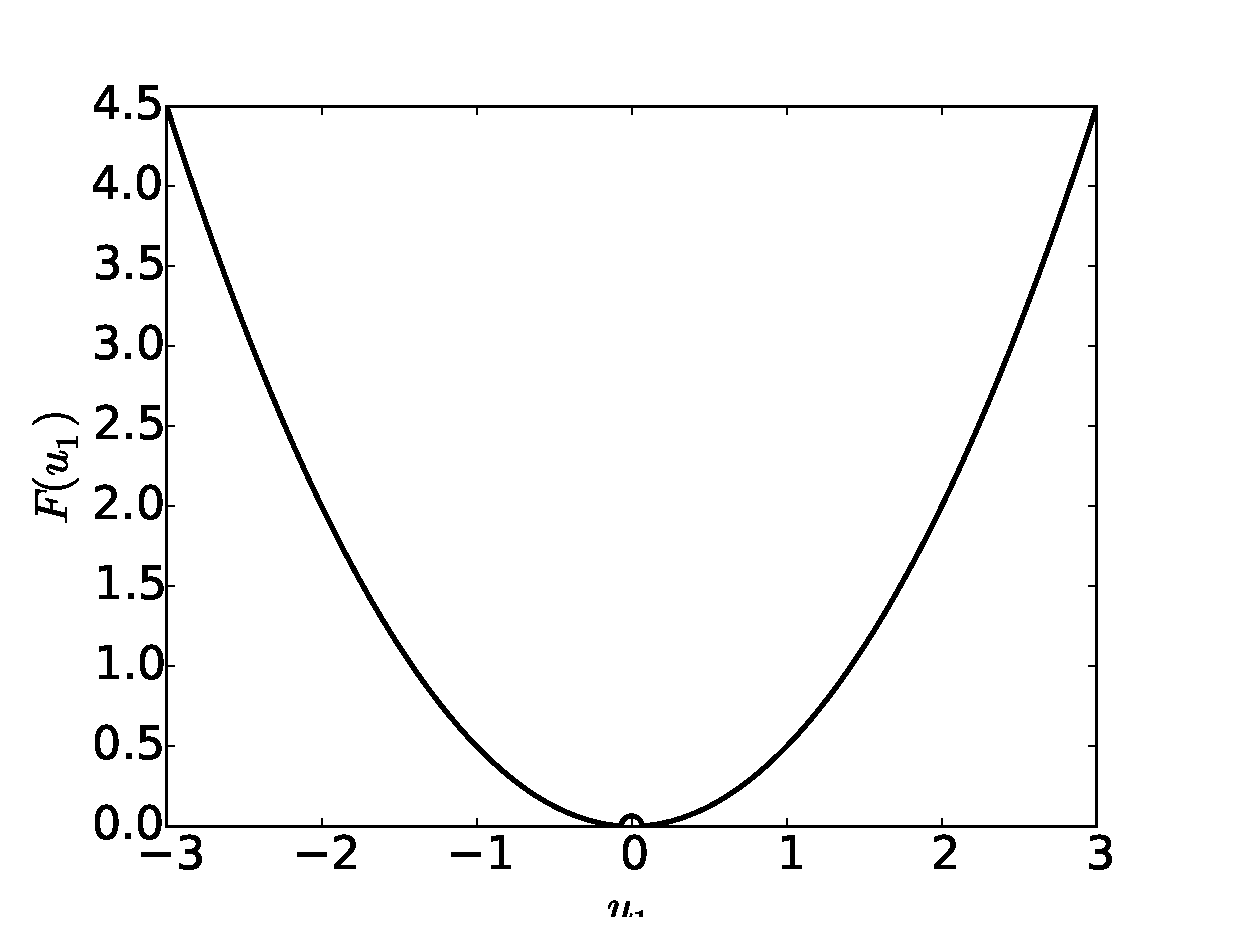
\includegraphics[width=8.0 cm]{figure/a10_lambda0.eps}
		\caption{$a=1.0,\ \lambda = 0.0$}
	\end{subfigure}
	\begin{subfigure}[h]{8.0 cm}
        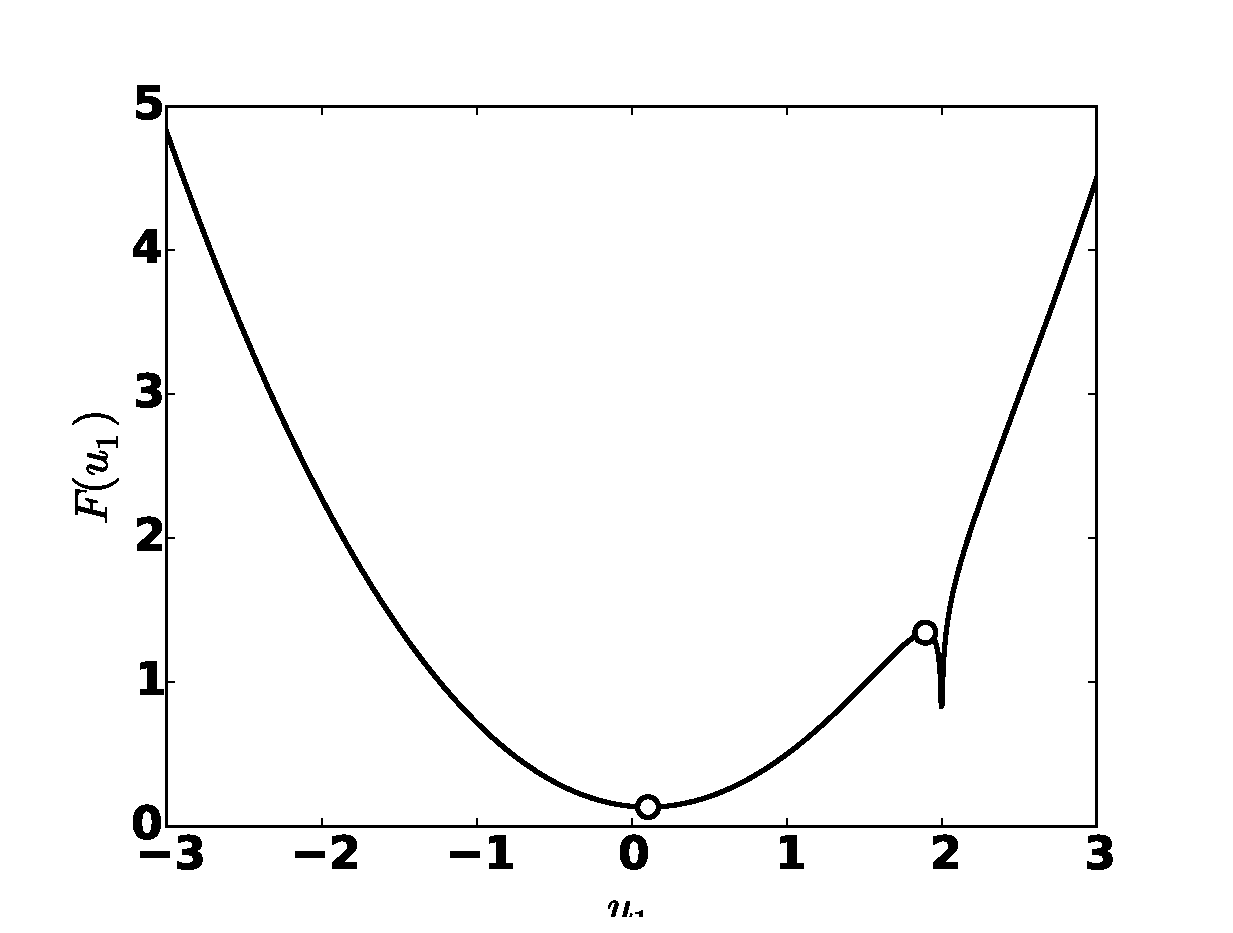
\includegraphics[width=8.0 cm]{figure/a20_lambda2.eps}
		\caption{$a=2.0,\ \lambda = 0.2$}
    \end{subfigure}
    \\
    \begin{subfigure}[h]{8.0 cm}
		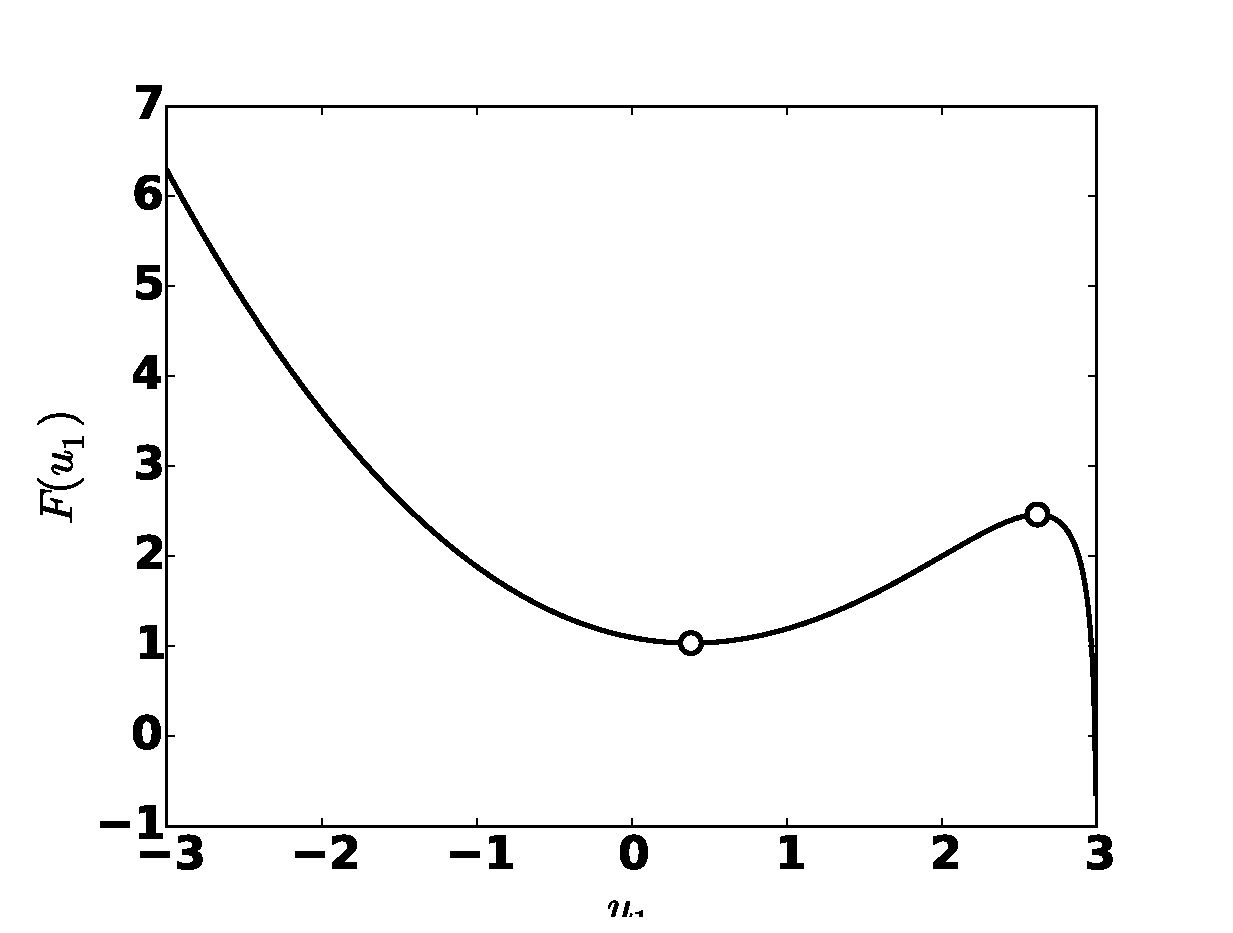
\includegraphics[width=8.0 cm]{figure/a30_lambda10.eps}
		\caption{$a=3.0,\ \lambda = 1.0$}
	\end{subfigure}
	\begin{subfigure}[h]{8.0 cm}
        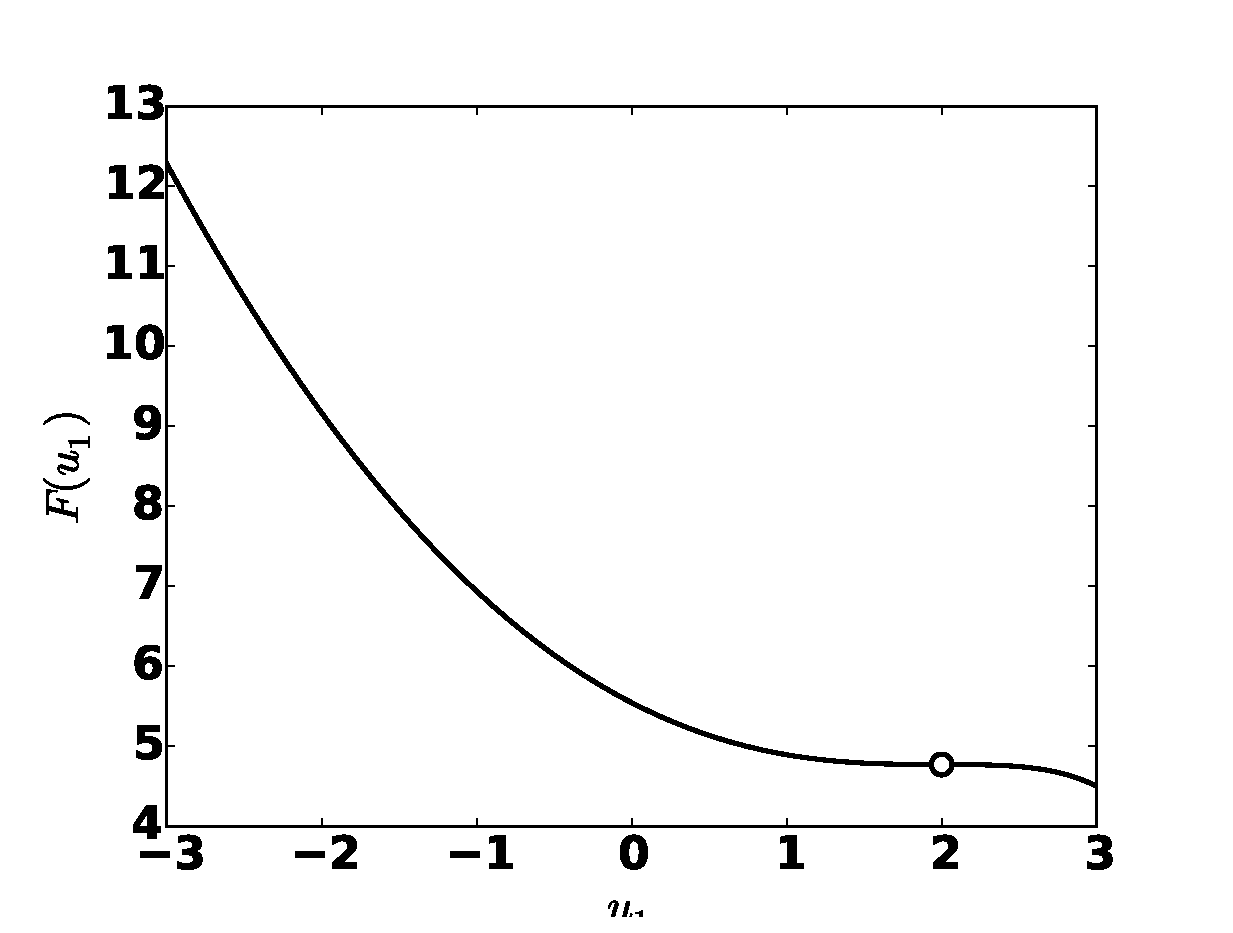
\includegraphics[width=8.0 cm]{figure/a40_lambda40.eps}
		\caption{$a=4.0,\ \lambda = 1.0$}
    \end{subfigure}
    \\
    	\begin{subfigure}[h]{8.0 cm}
        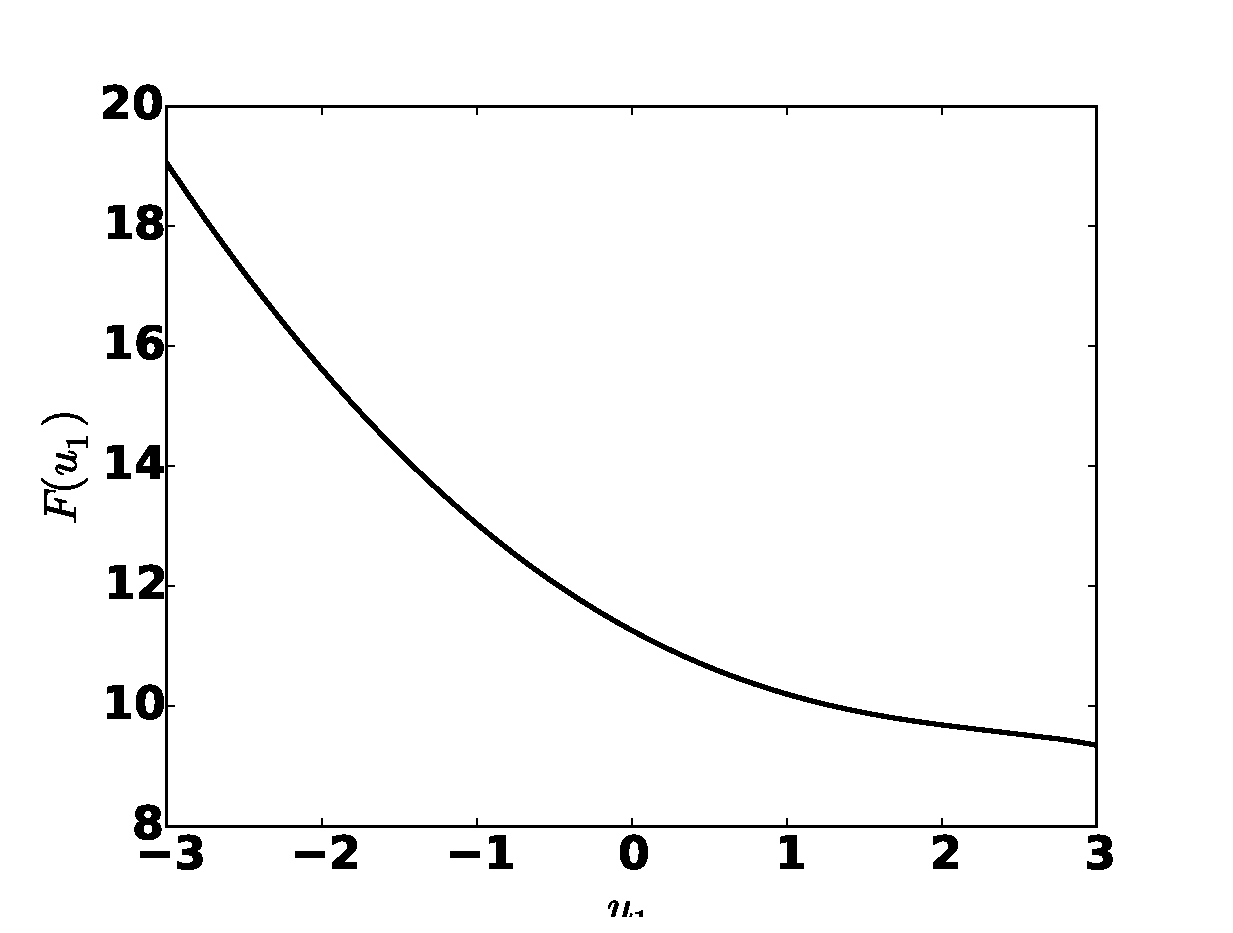
\includegraphics[width=8.0 cm]{figure/a50_lambda70.eps}
		\caption{$a=5.0,\ \lambda = 7.0$}
    \end{subfigure}
    \caption{Potential energy vs. displacement for different values of $a$ and $\lambda$. The white circle corresponds to the equilibrium point of the system.}
    \label{fig:potentialFunction}
\end{figure}
%
%
\begin{figure}[H]
	\centering
	\begin{subfigure}[h]{8.0 cm}
		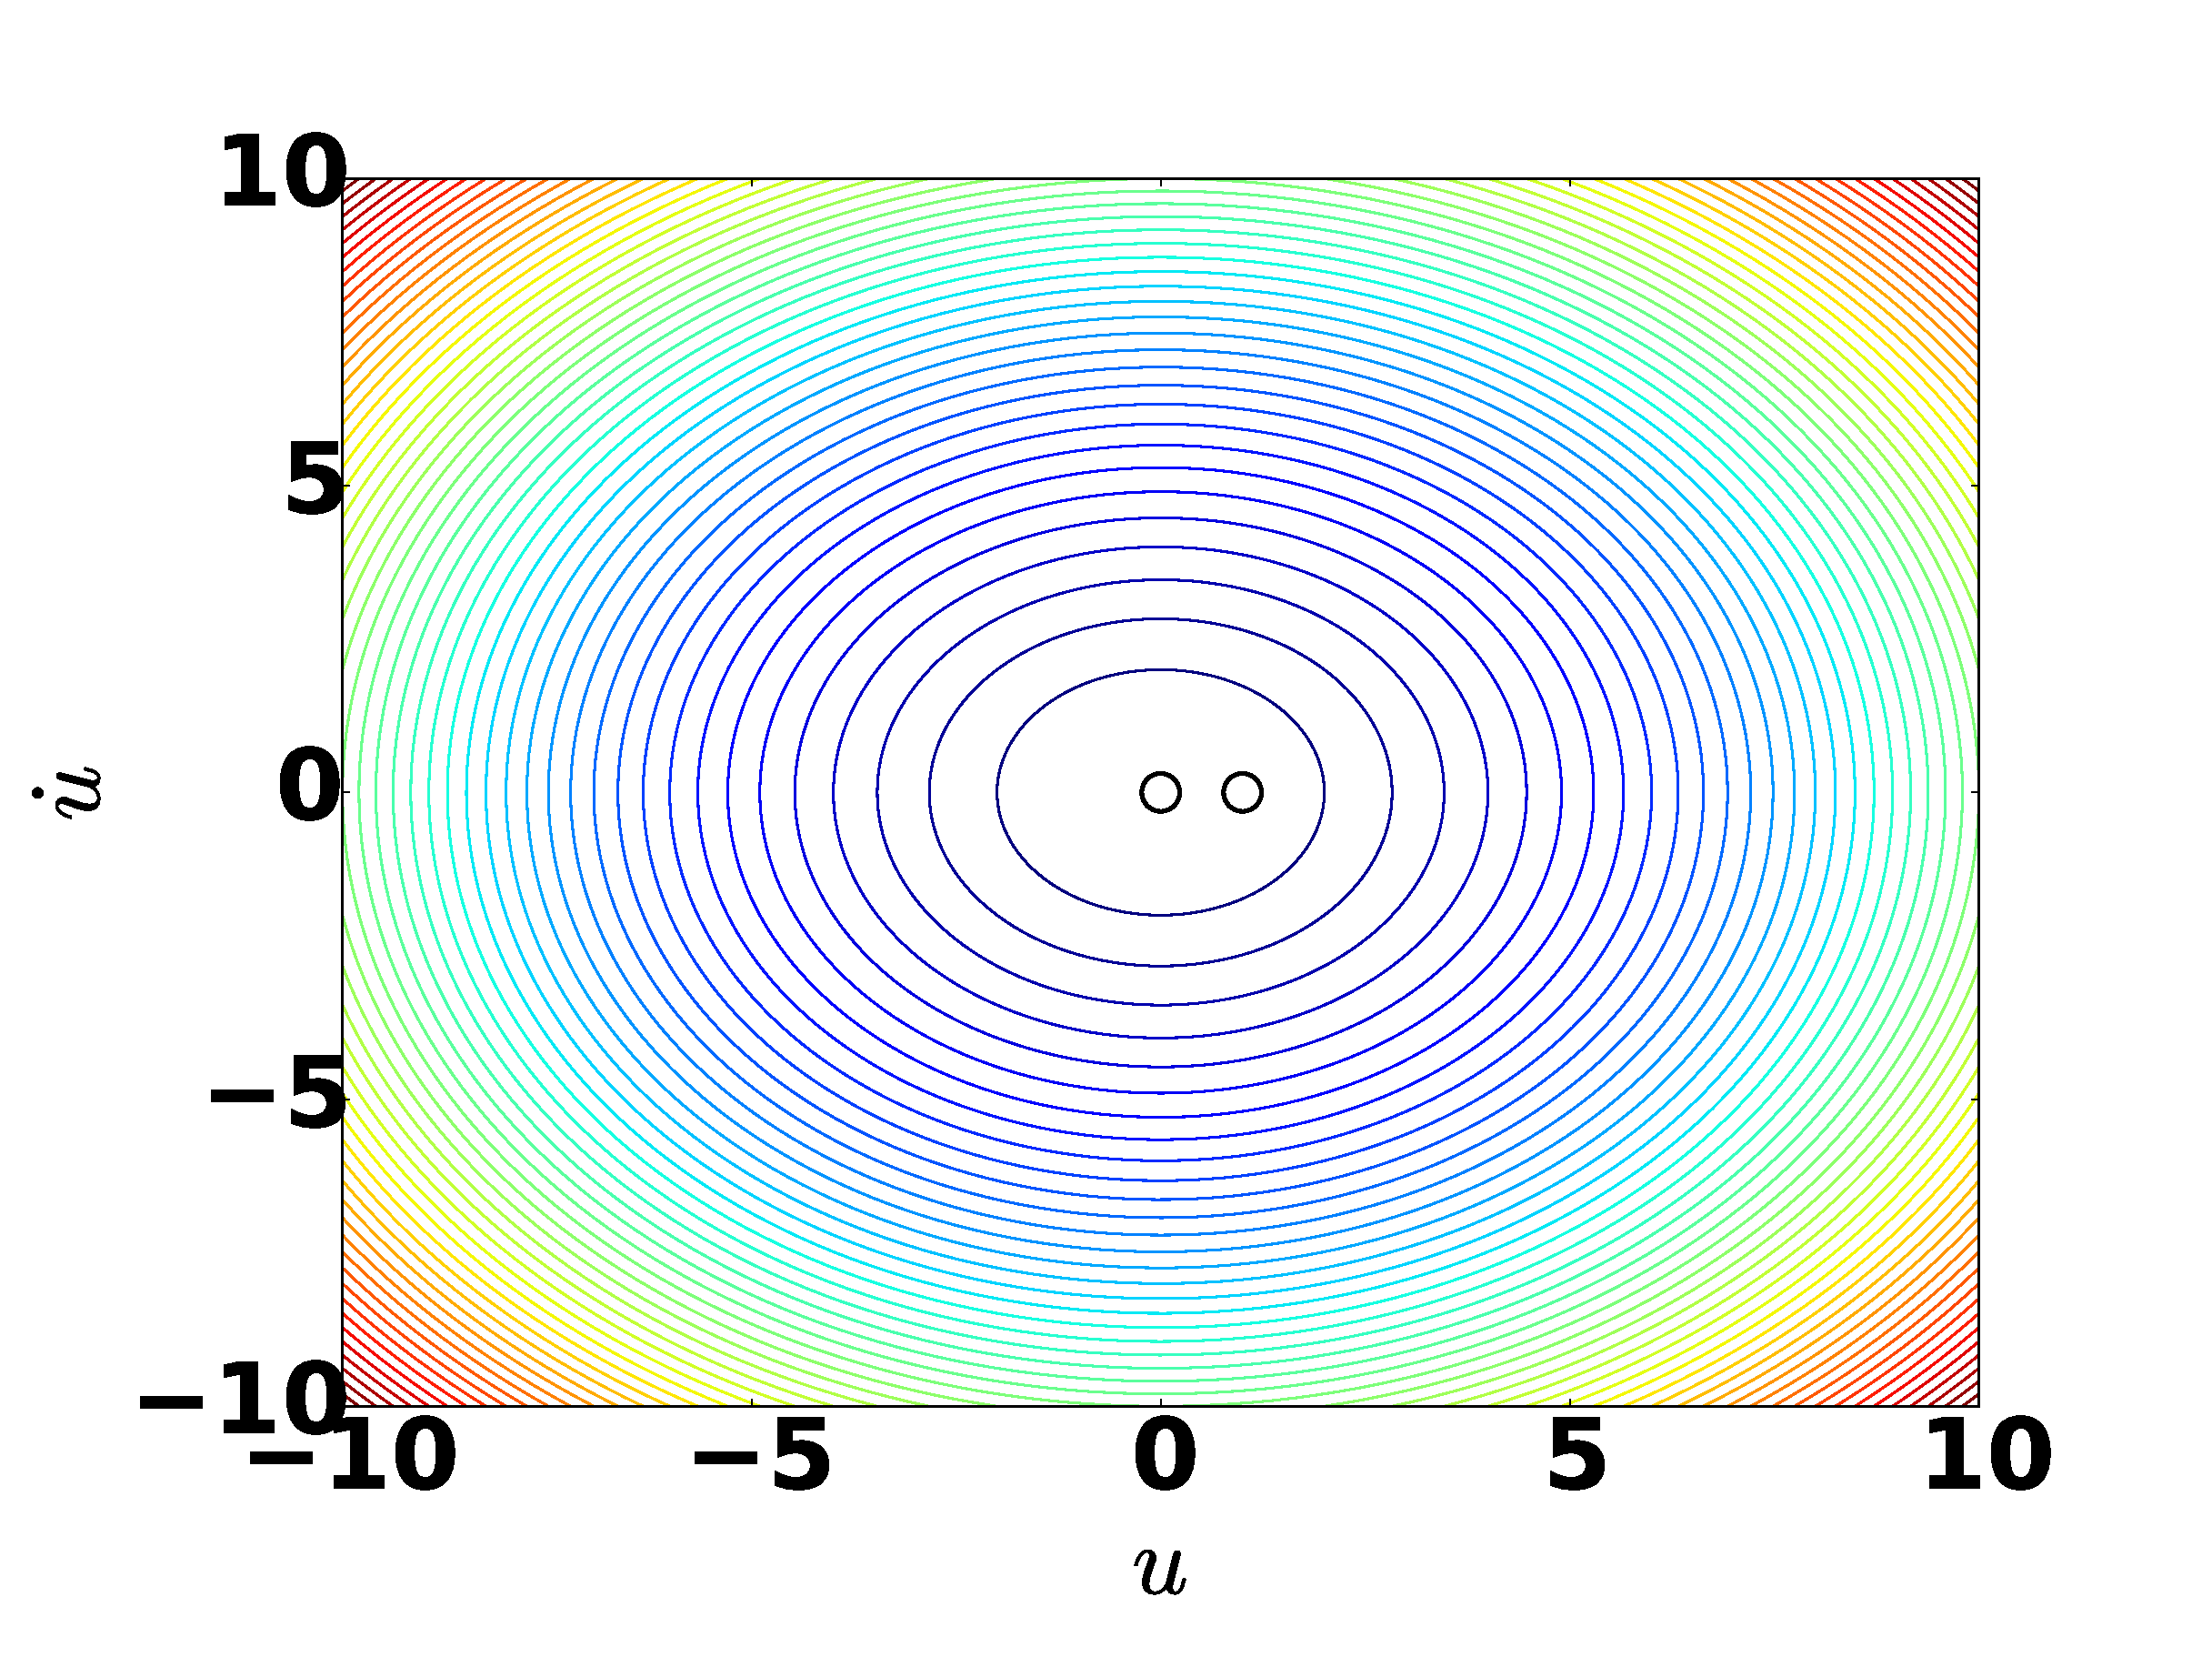
\includegraphics[width=8.0 cm]{figure/mechanical_a10_lambda0.eps}
		\caption{$a=1.0,\ \lambda = 0.0$}
	\end{subfigure}
	\begin{subfigure}[h]{8.0 cm}
        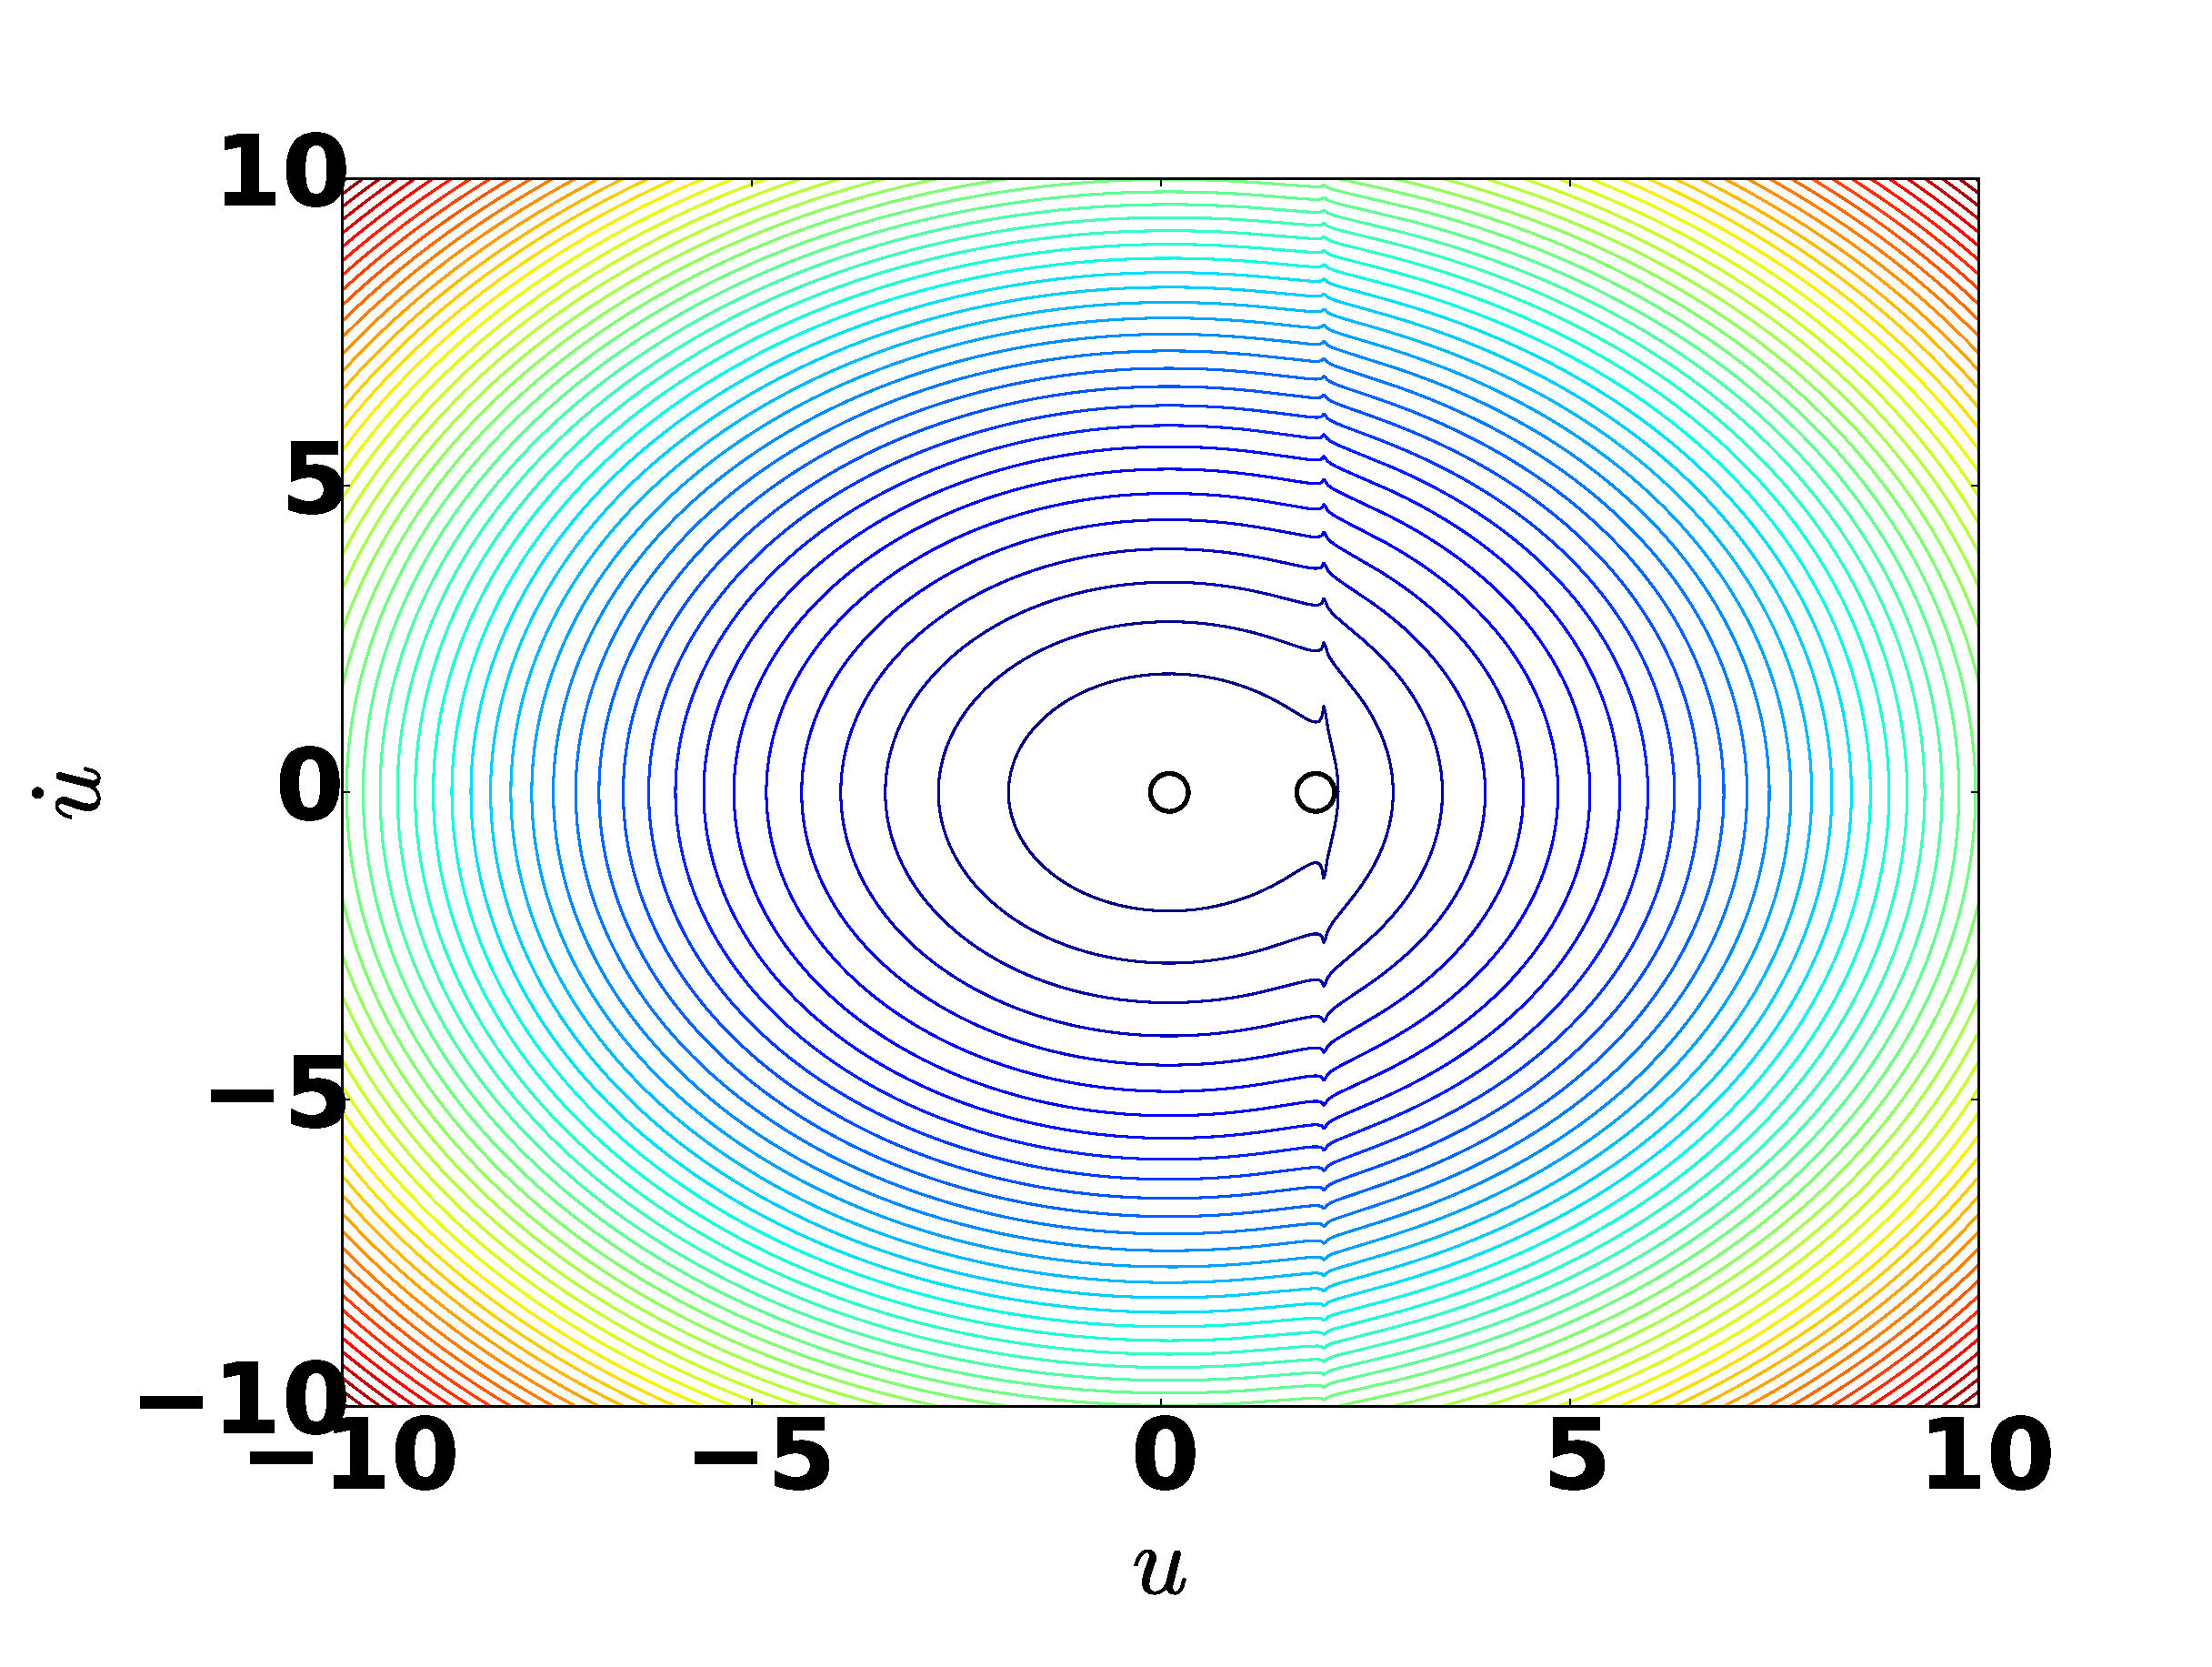
\includegraphics[width=8.0 cm]{figure/mechanical_a20_lambda2.eps}
		\caption{$a=2.0,\ \lambda = 0.2$}
    \end{subfigure}
    \\
    \begin{subfigure}[h]{8.0 cm}
		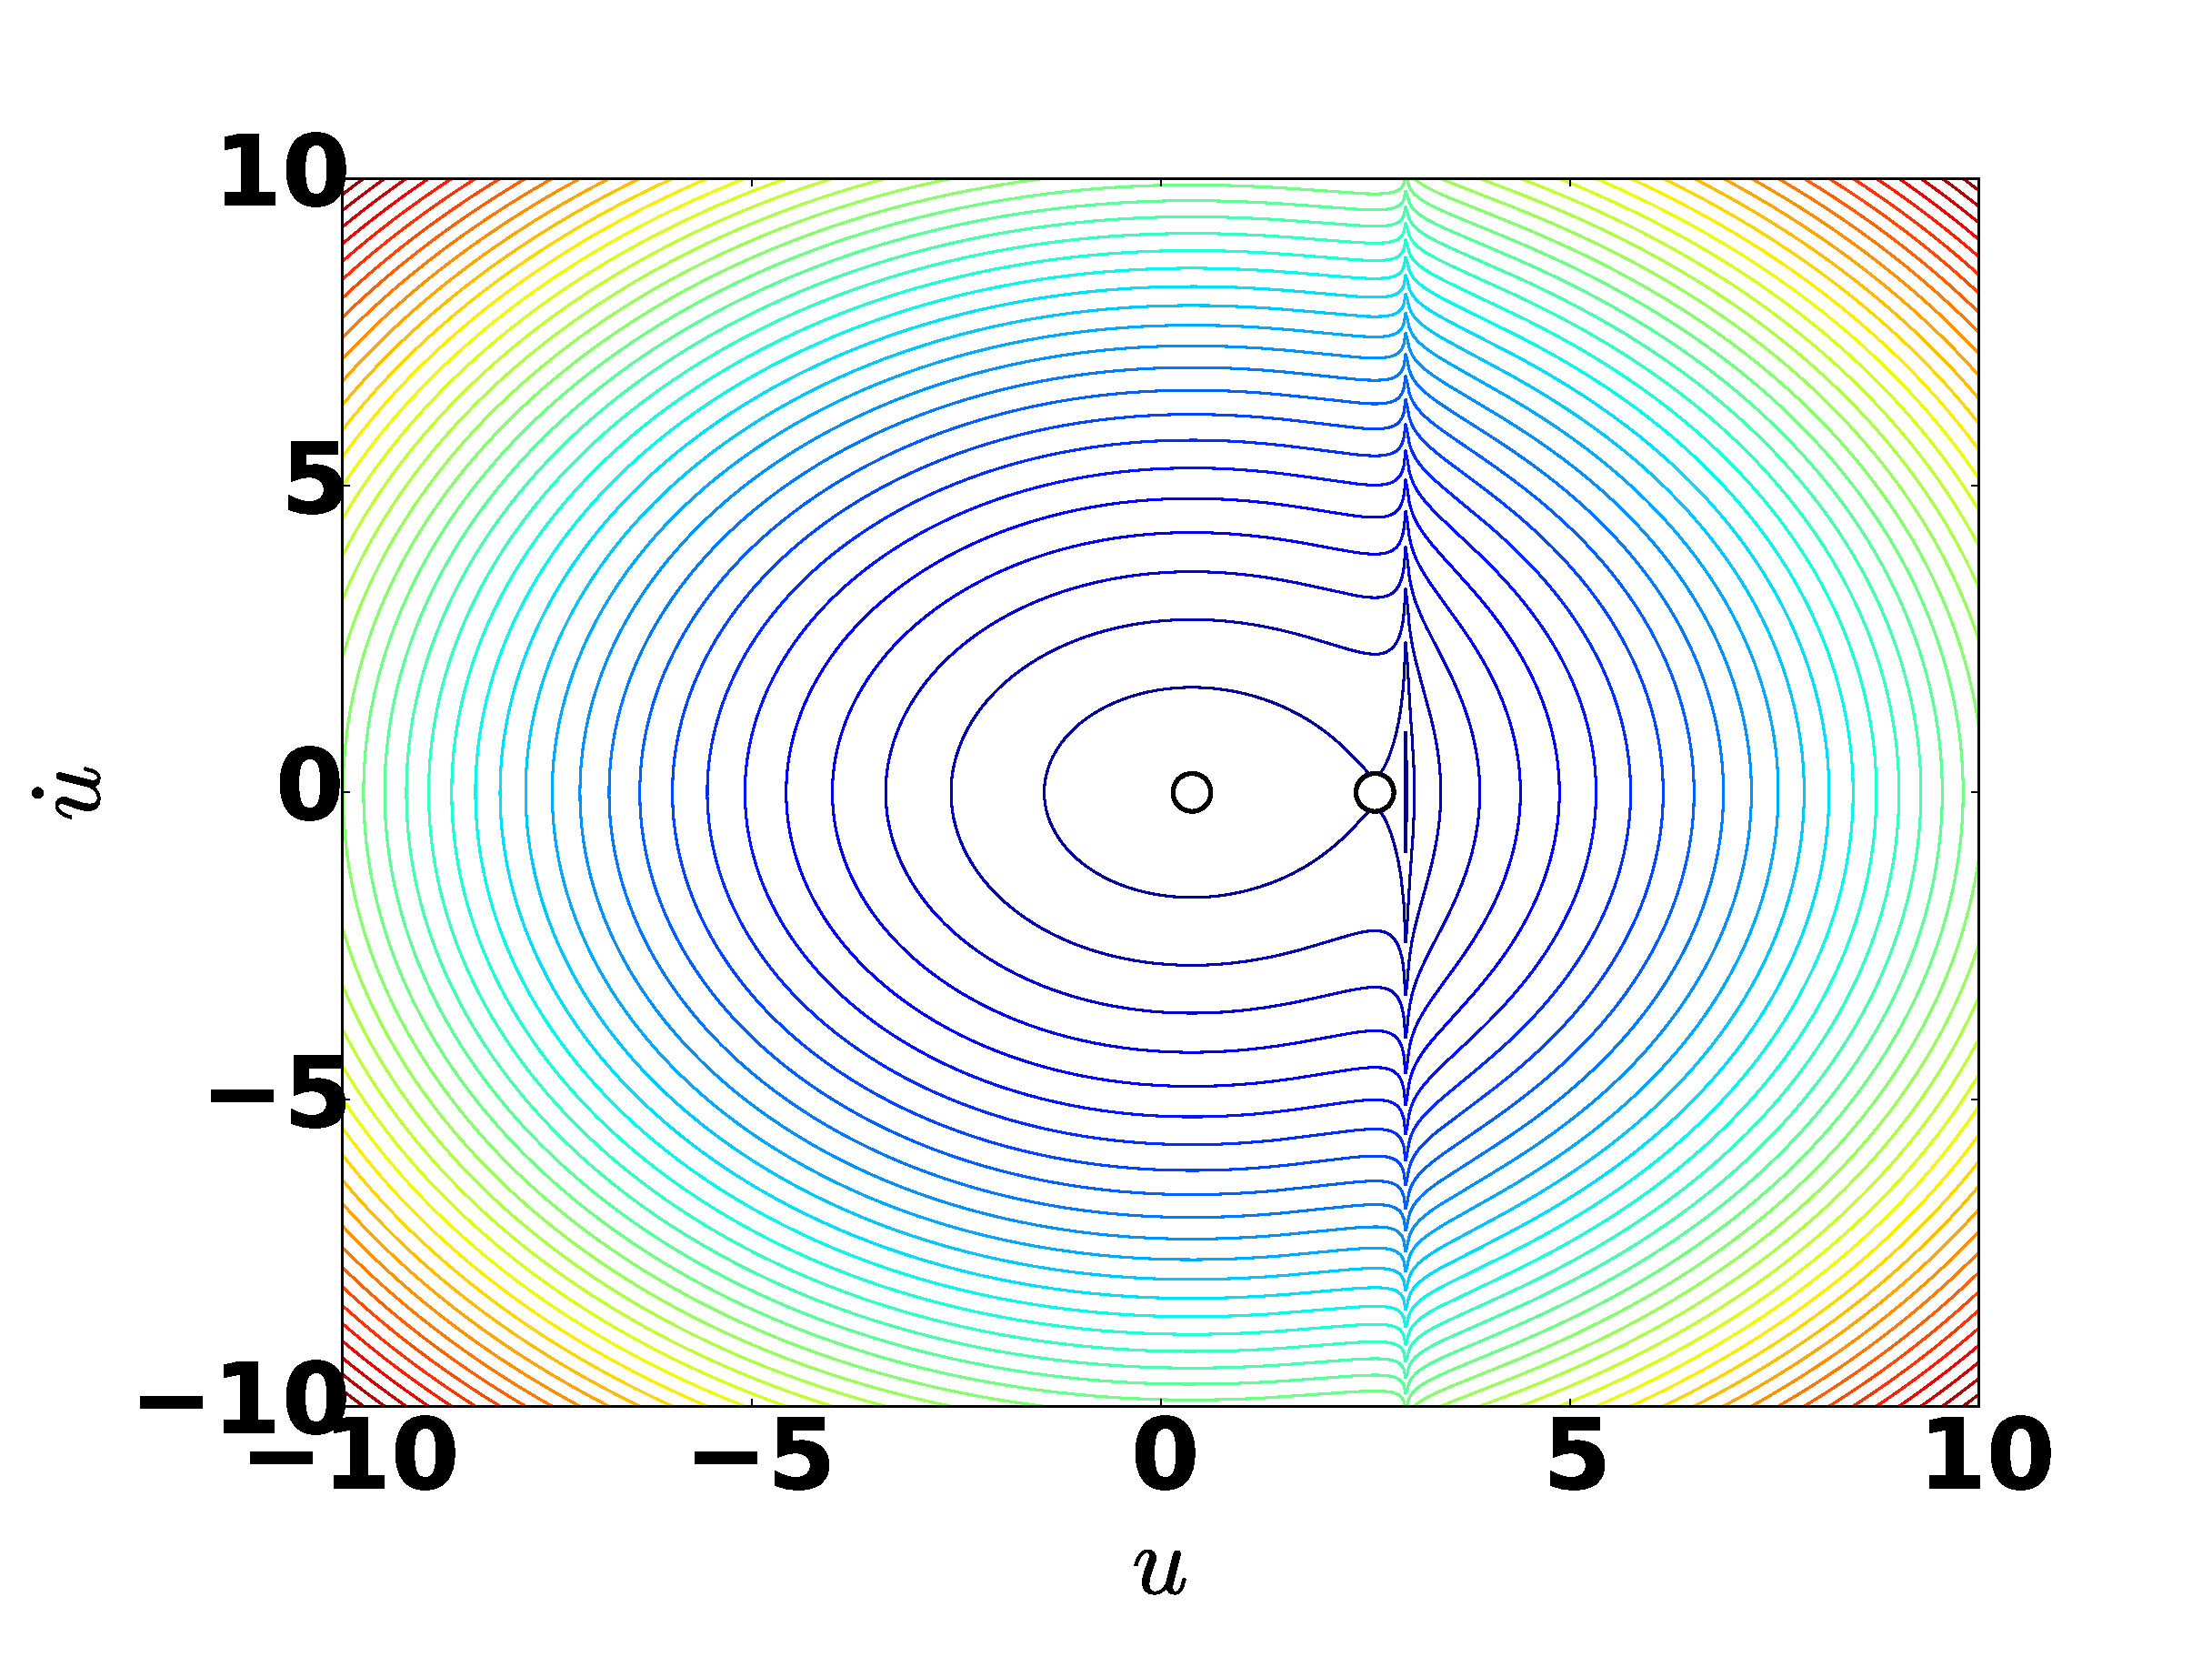
\includegraphics[width=8.0 cm]{figure/mechanical_a30_lambda10.eps}
		\caption{$a=3.0,\ \lambda = 1.0$}
	\end{subfigure}
	\begin{subfigure}[h]{8.0 cm}
        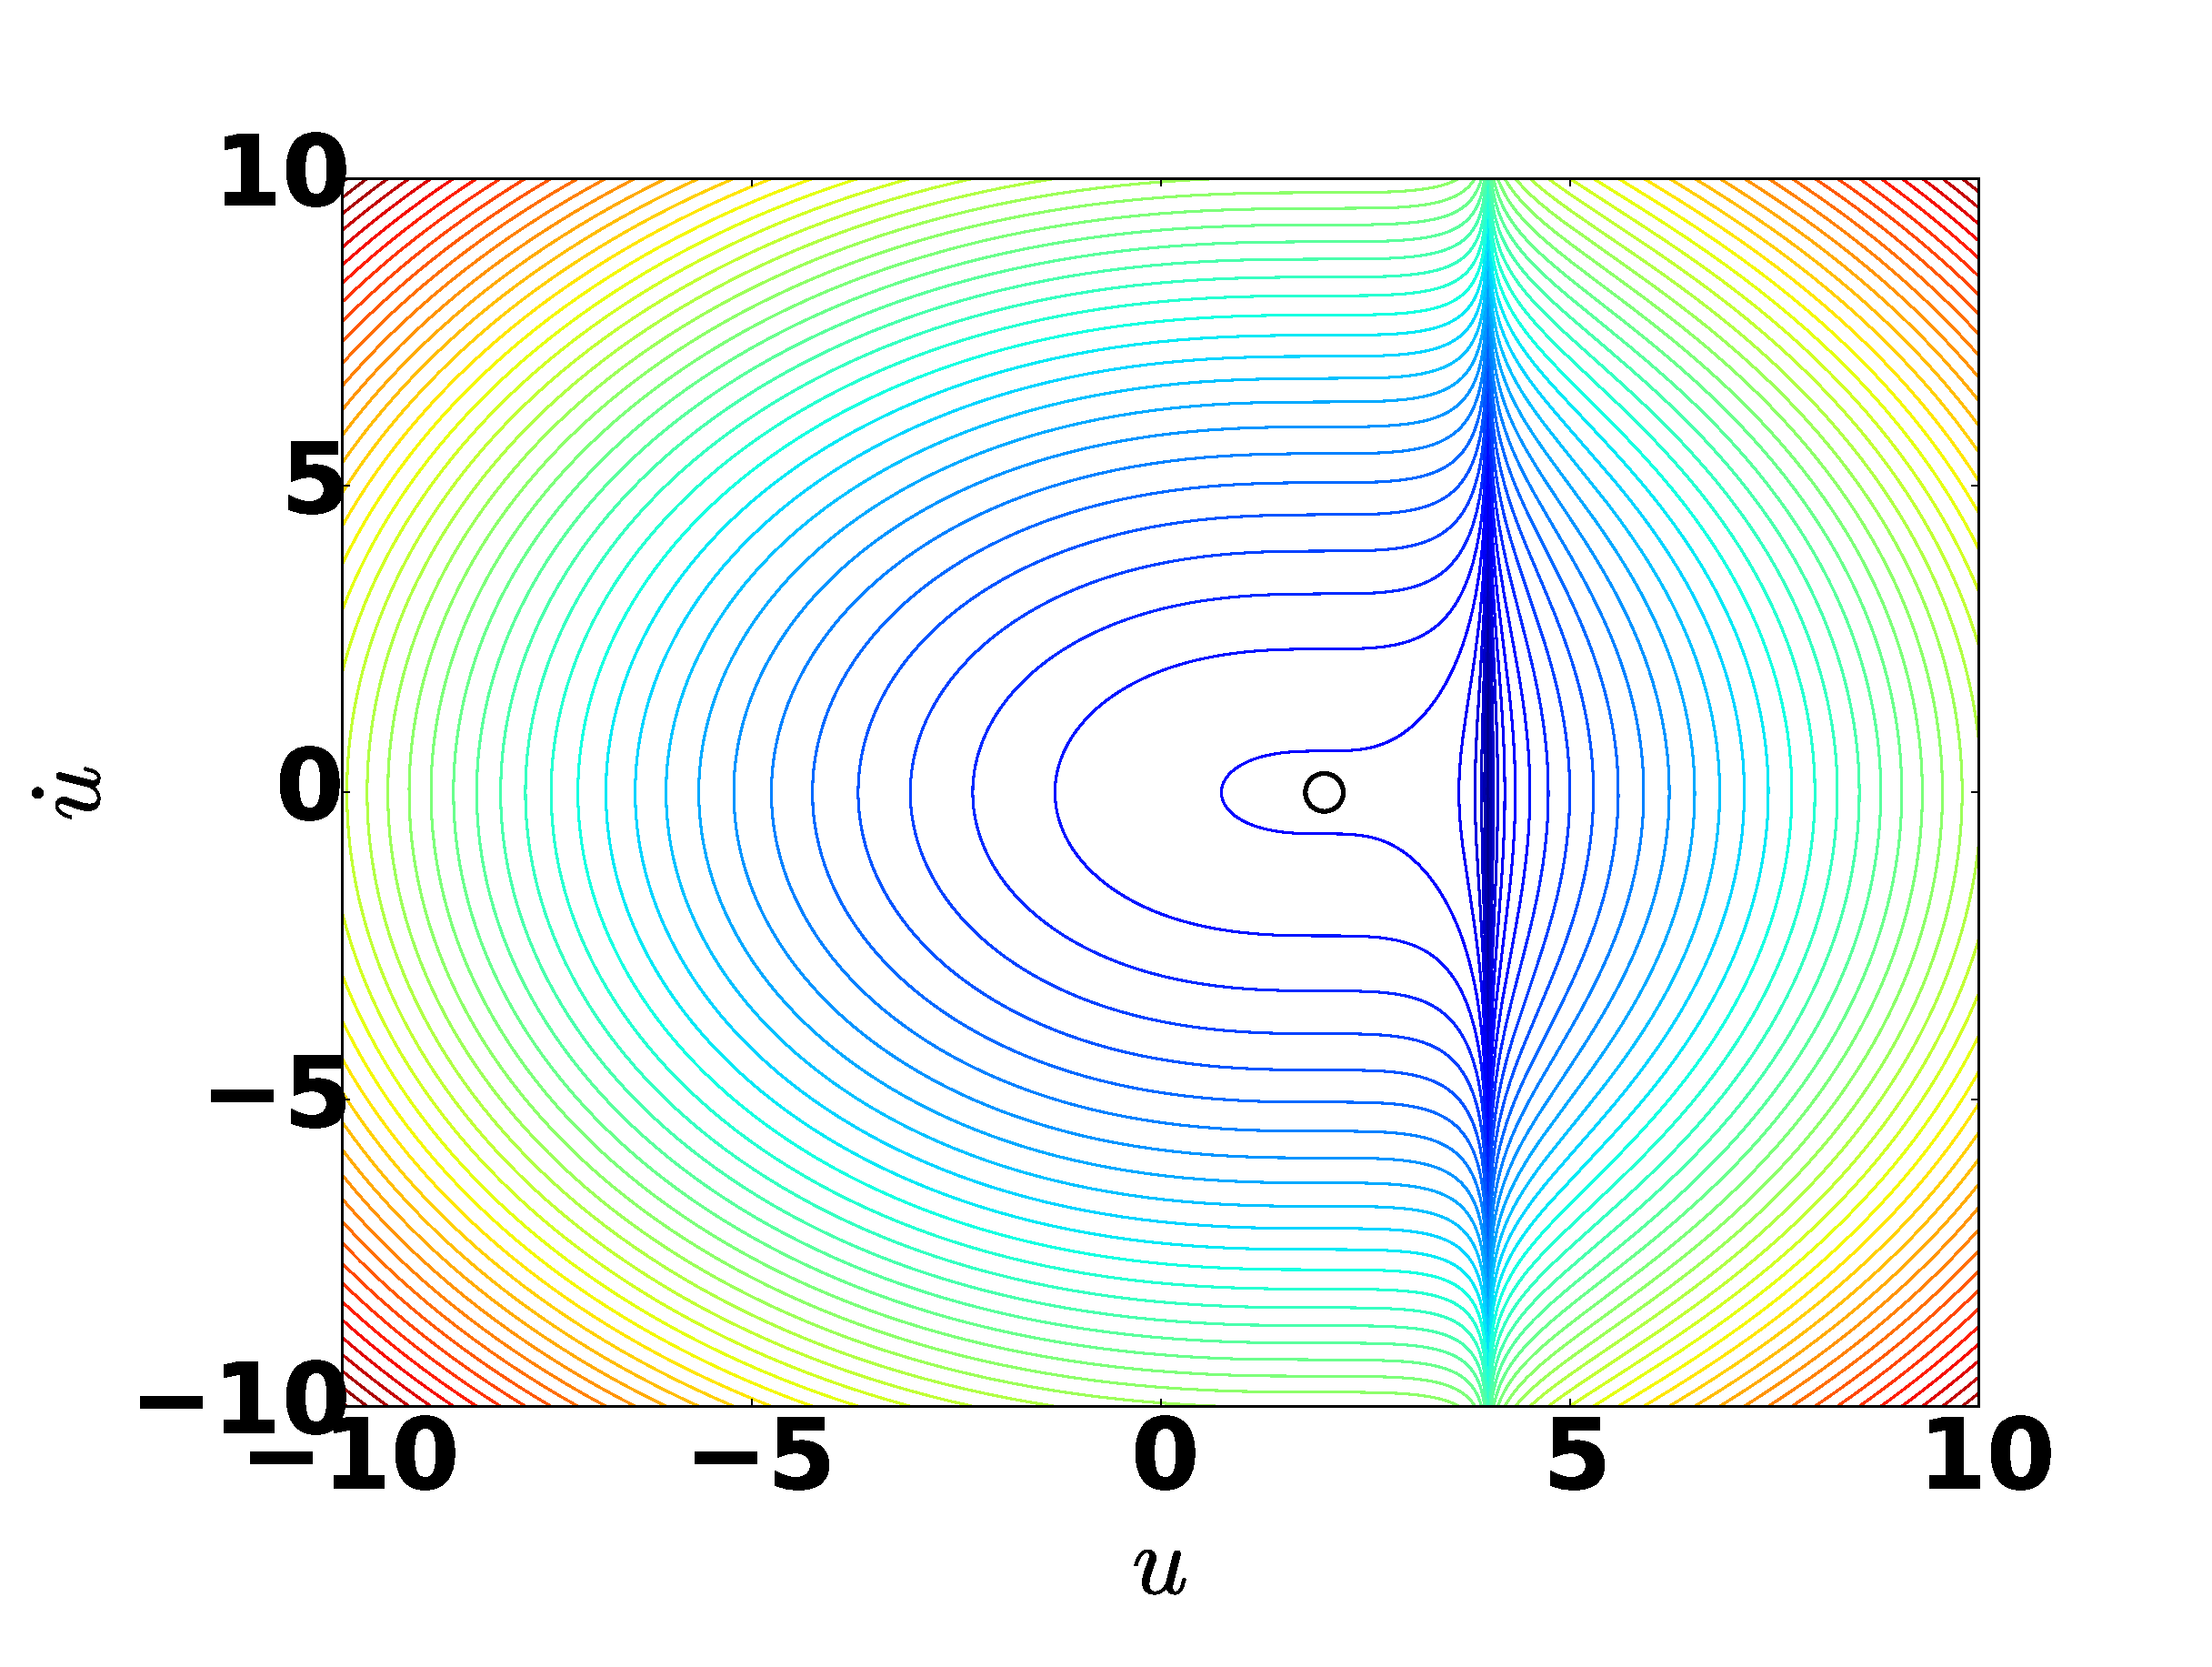
\includegraphics[width=8.0 cm]{figure/mechanical_a40_lambda40.eps}
		\caption{$a=4.0,\ \lambda = 1.0$}
    \end{subfigure}
    \\
    	\begin{subfigure}[h]{8.0 cm}
        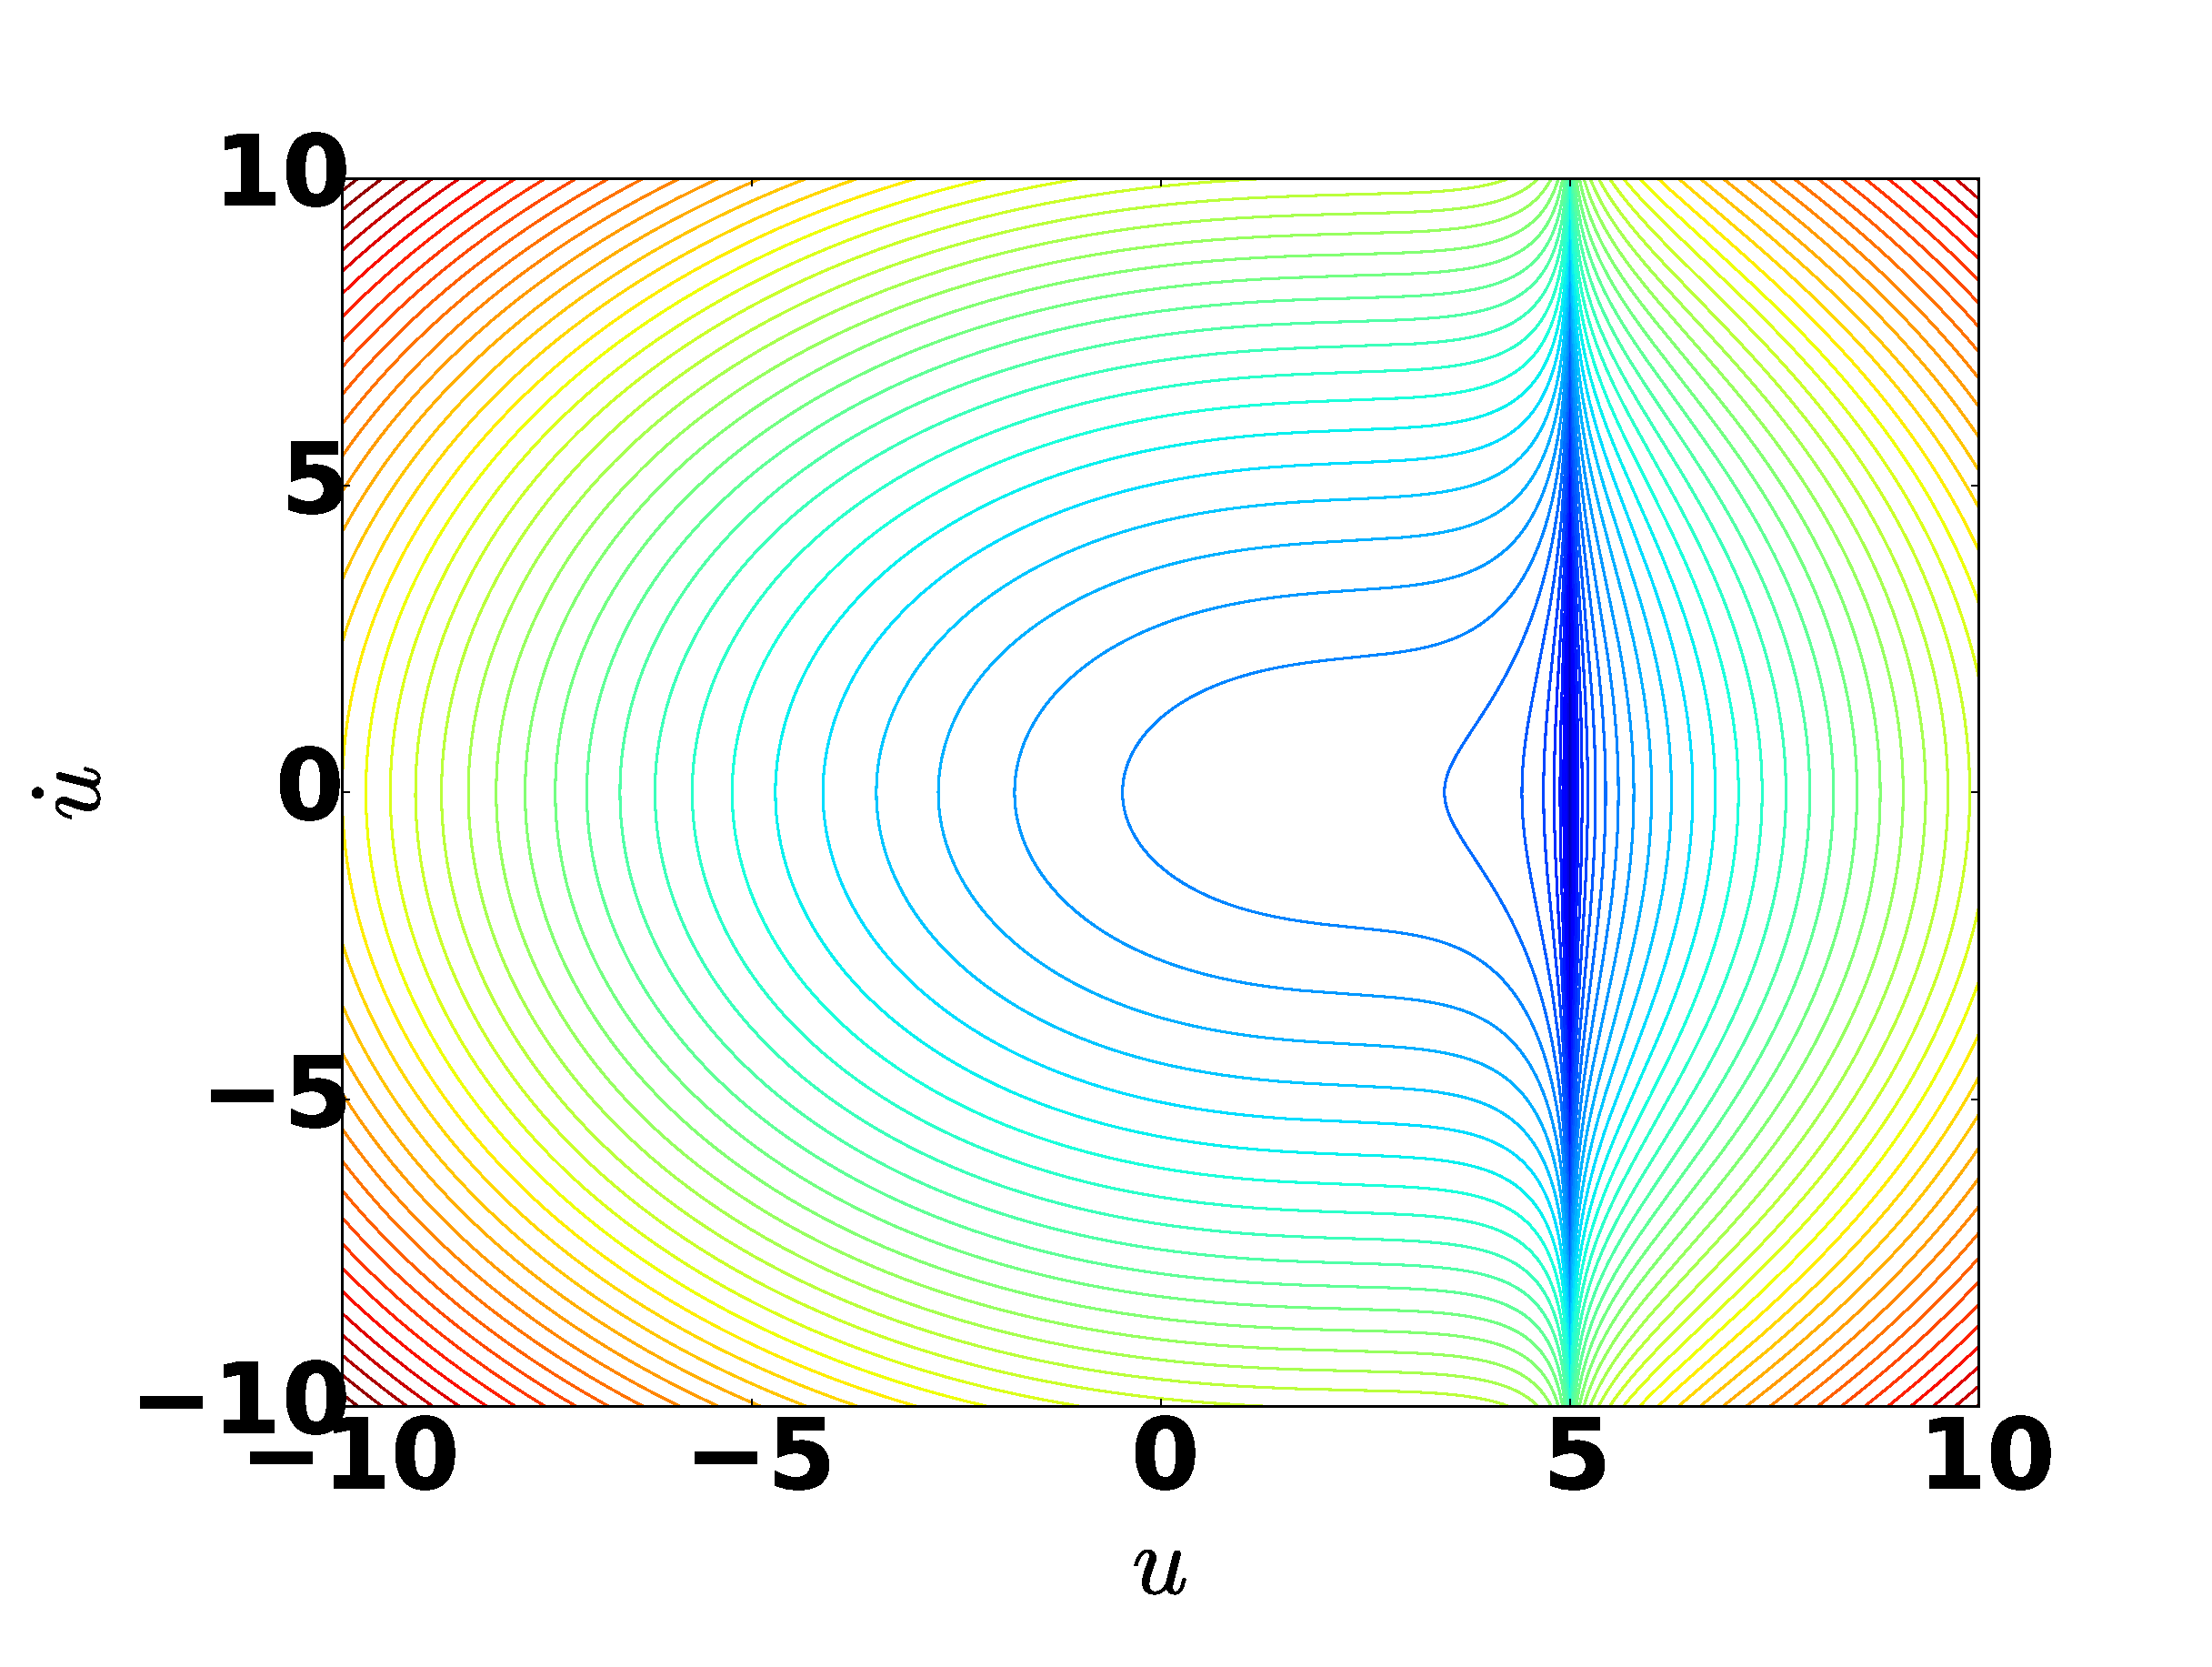
\includegraphics[width=8.0 cm]{figure/mechanical_a50_lambda70.eps}
		\caption{$a=5.0,\ \lambda = 7.0$}
    \end{subfigure}
    \caption{Contour plots of total mechanical energy (potential + kinetic energy) for different values of $a$ and $\lambda$. The white circle corresponds to the equilibrium point of the system.}
    \label{fig:potentialFunction}
\end{figure}
%
To draw the phase plot, the equation of motion needs to put into the state form. This is done by defining new variable $u_1$ and $u_2$ and rewriting Equation \eqref{eq:equationOfMotion} in the following form.
%
\begin{equation}\label{eq:stateEquation}
	\begin{cases}
    \dot{u}_1 = u_2 \\
    \dot{u}_2 = -u_1 + \dfrac{\lambda}{a - u_1}
	\end{cases}
\end{equation}
%
The phase plot ($\dot{u}$ vs. $u$) of this system is shown in Figure \ref{fig:phasePlot}. The lines represents different trajectories of the solution for different boundary condition. These are calculated by integrating Equation \eqref{eq:stateEquation} using \texttt{odeint} function in \texttt{Python}.
%
\begin{figure}[H]
	\centering
	\begin{subfigure}[h]{8.0 cm}
		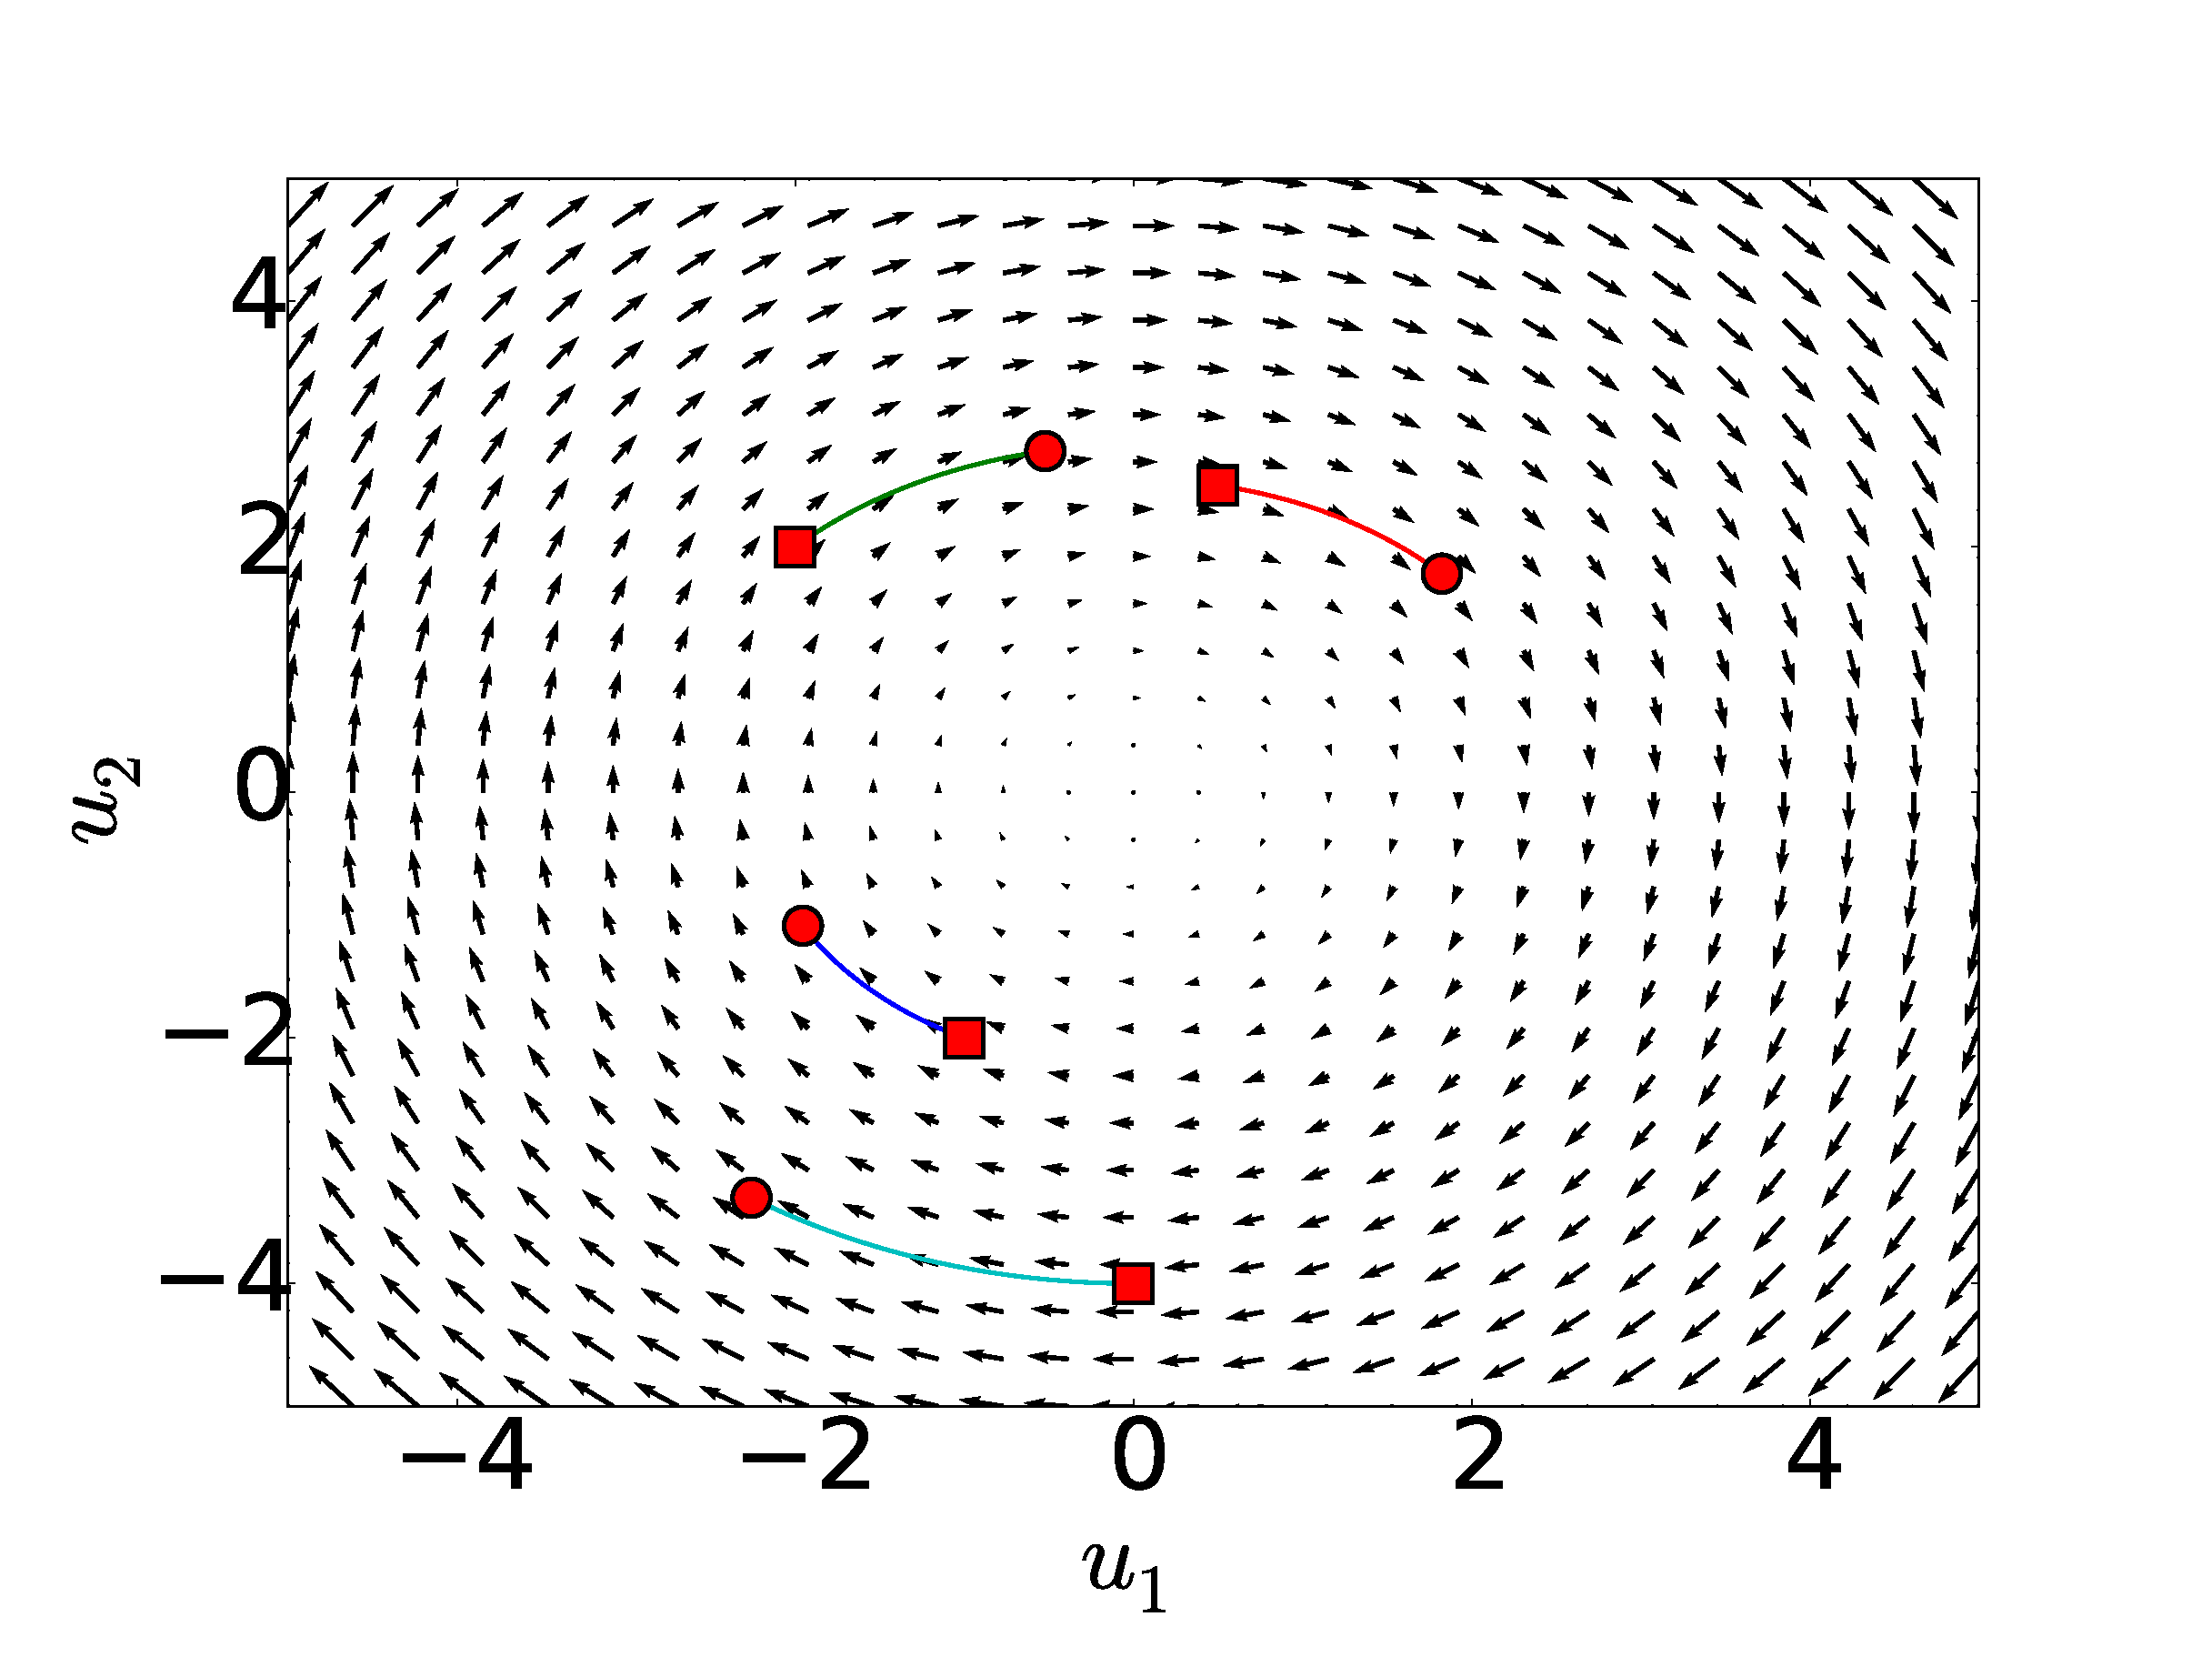
\includegraphics[width=8.0 cm]{figure/phase_a40_lambda0.eps}
		\caption{$a=4.0,\ \lambda = 0.0$}
	\end{subfigure}
	\begin{subfigure}[h]{8.0 cm}
        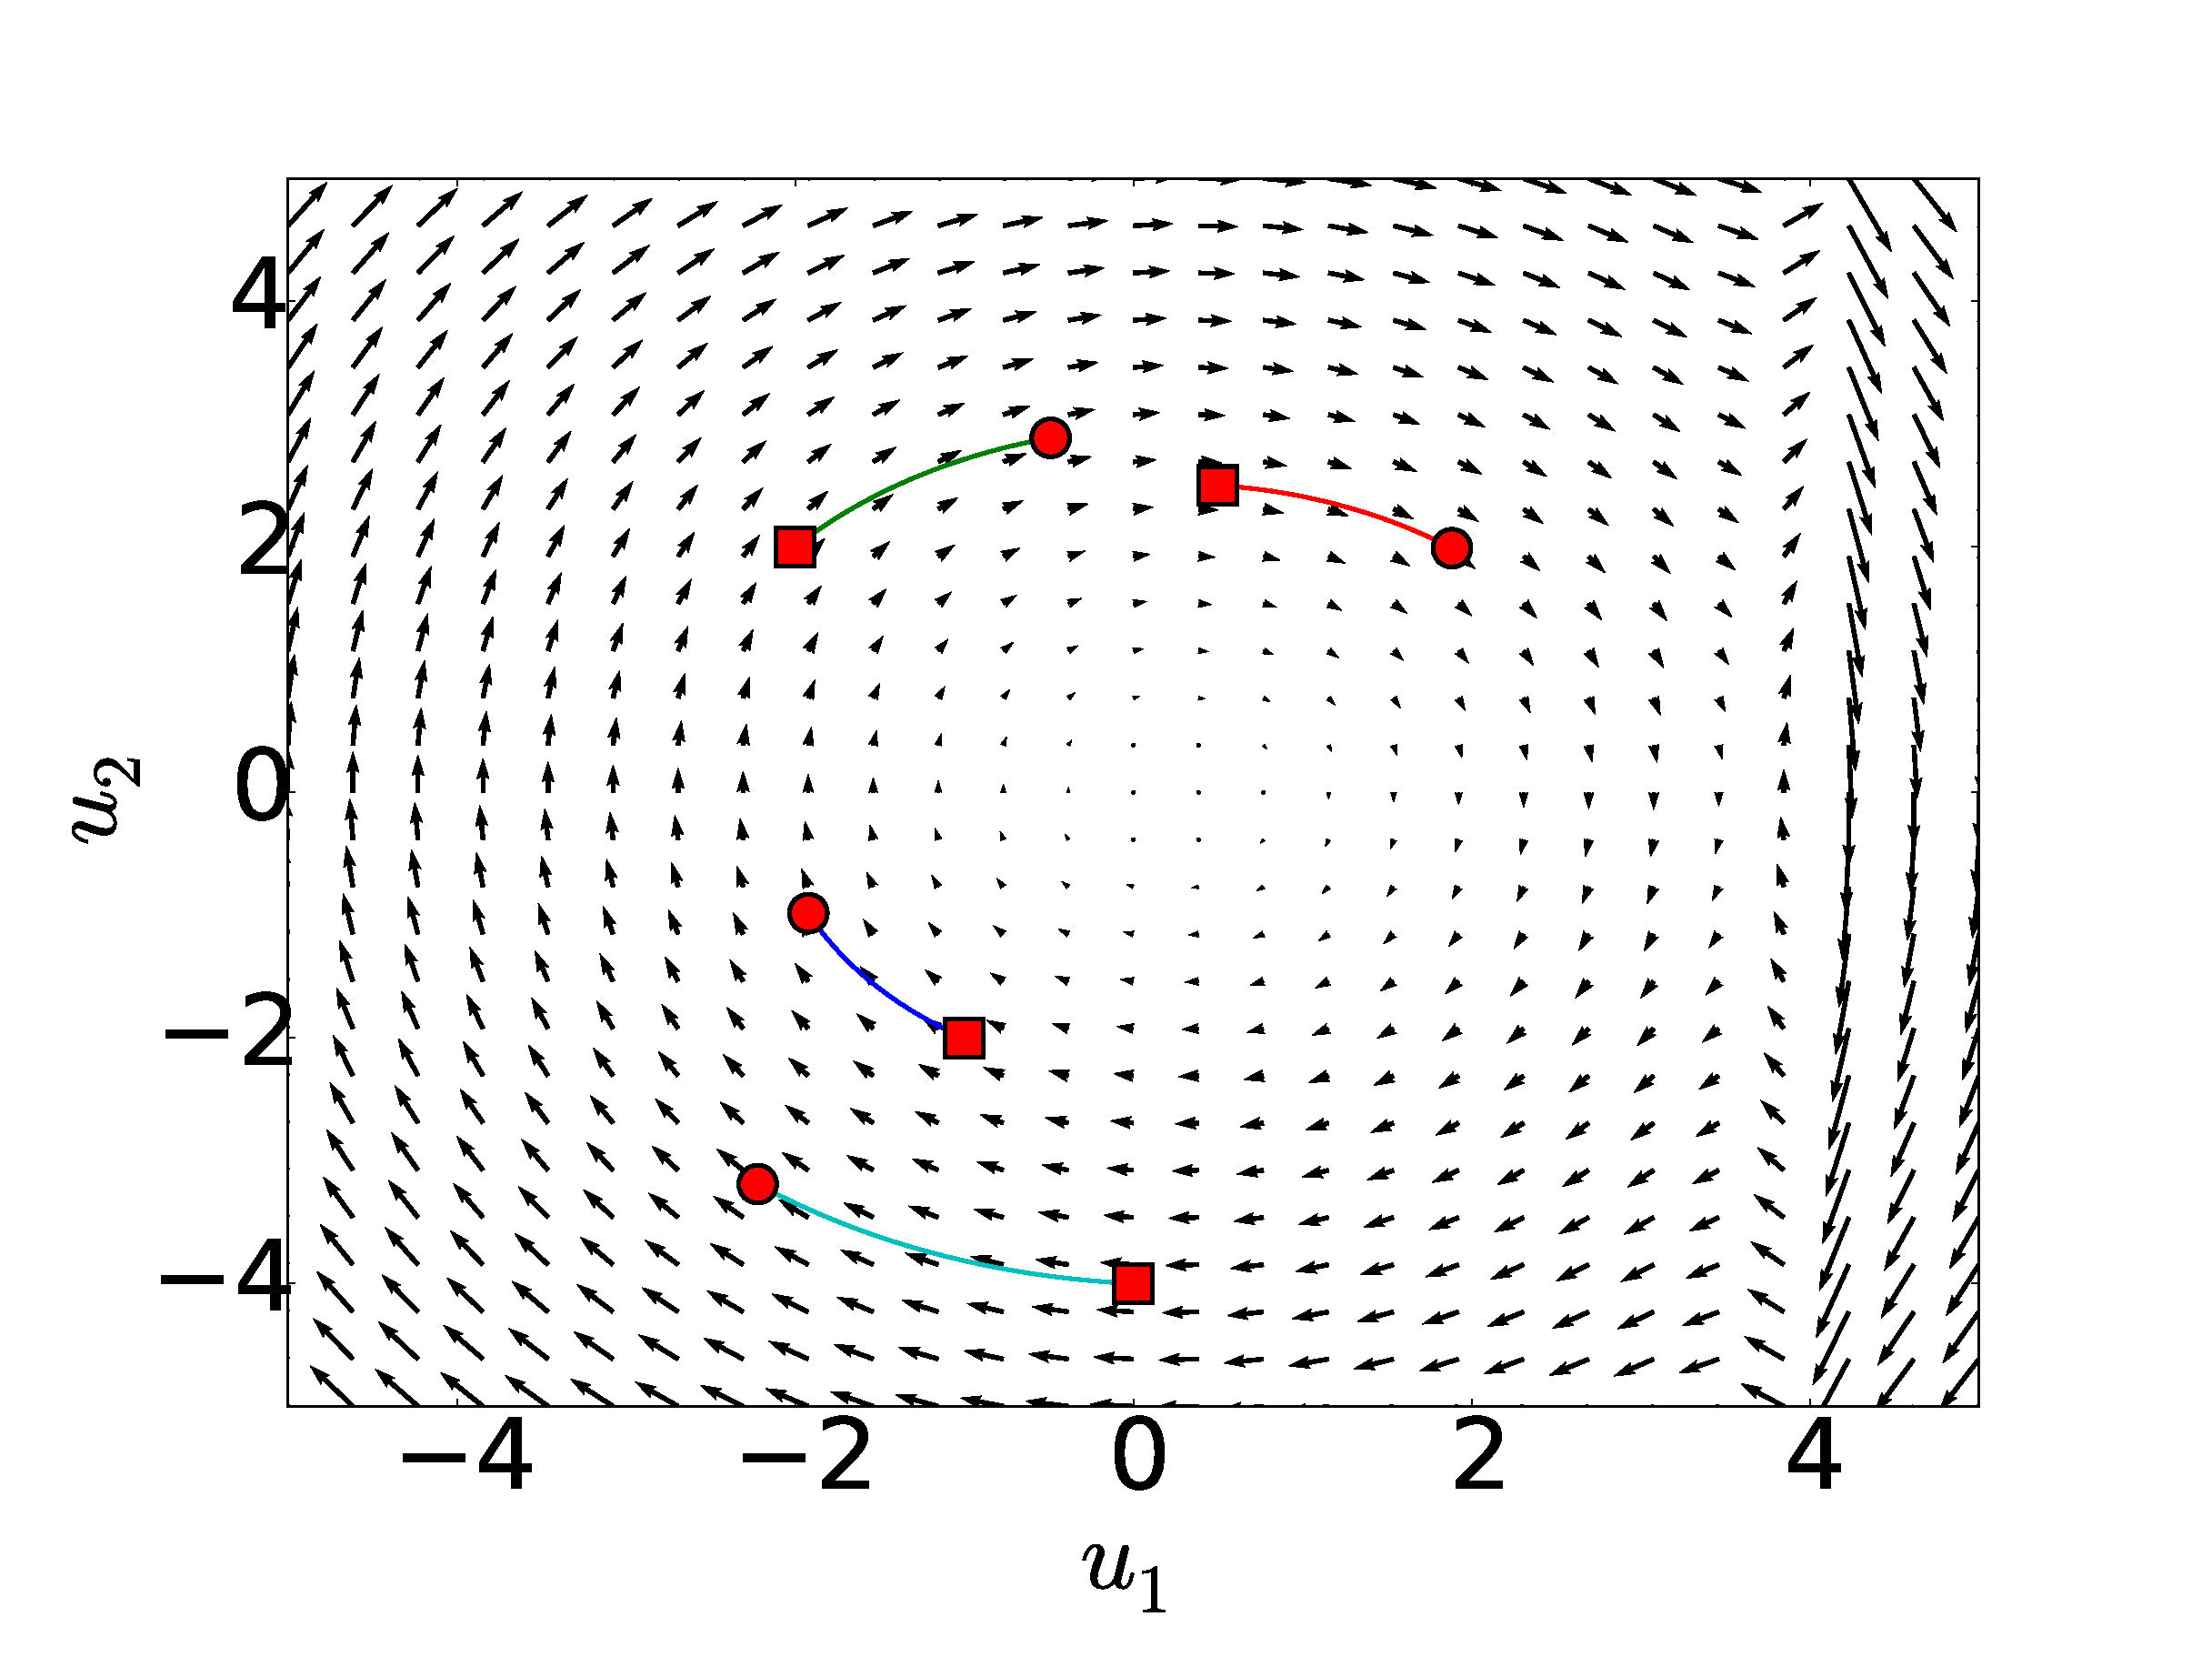
\includegraphics[width=8.0 cm]{figure/phase_a40_lambda10.eps}
		\caption{$a=4.0,\ \lambda = 1.0$}
    \end{subfigure}
    \\
    \begin{subfigure}[h]{8.0 cm}
		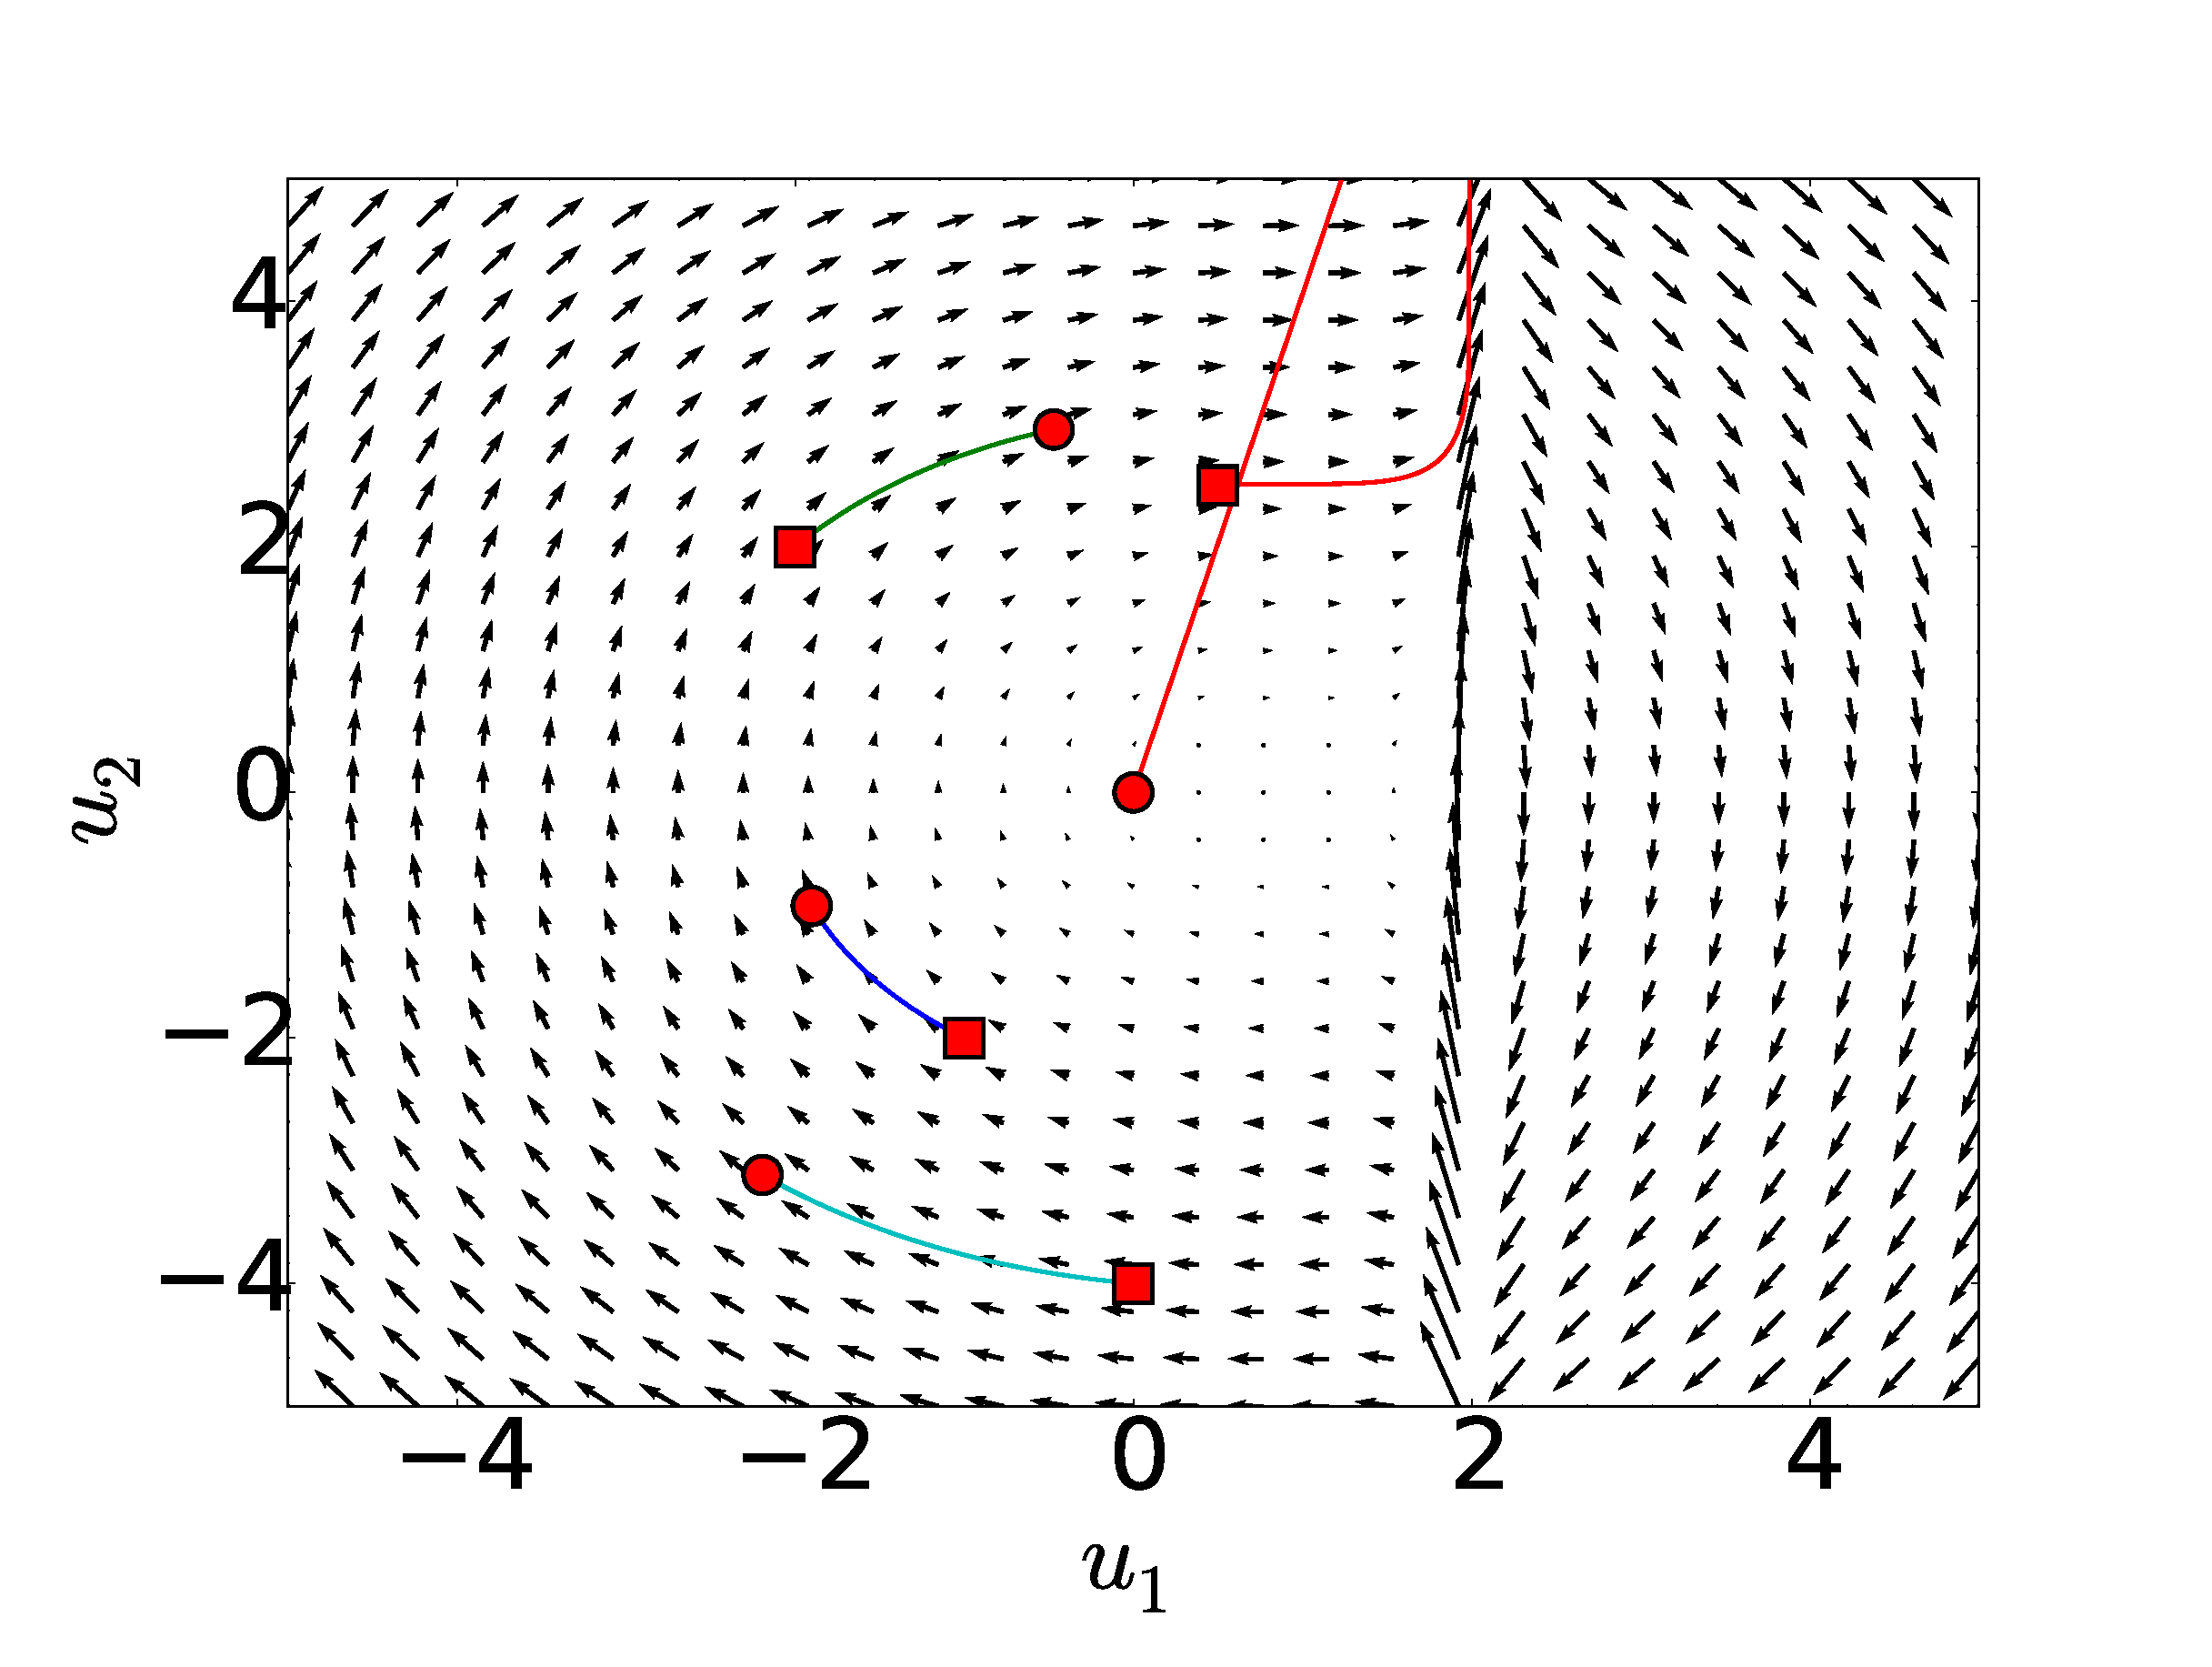
\includegraphics[width=8.0 cm]{figure/phase_a20_lambda10.eps}
		\caption{$a=2.0,\ \lambda = 1.0$}
	\end{subfigure}
	\begin{subfigure}[h]{8.0 cm}
        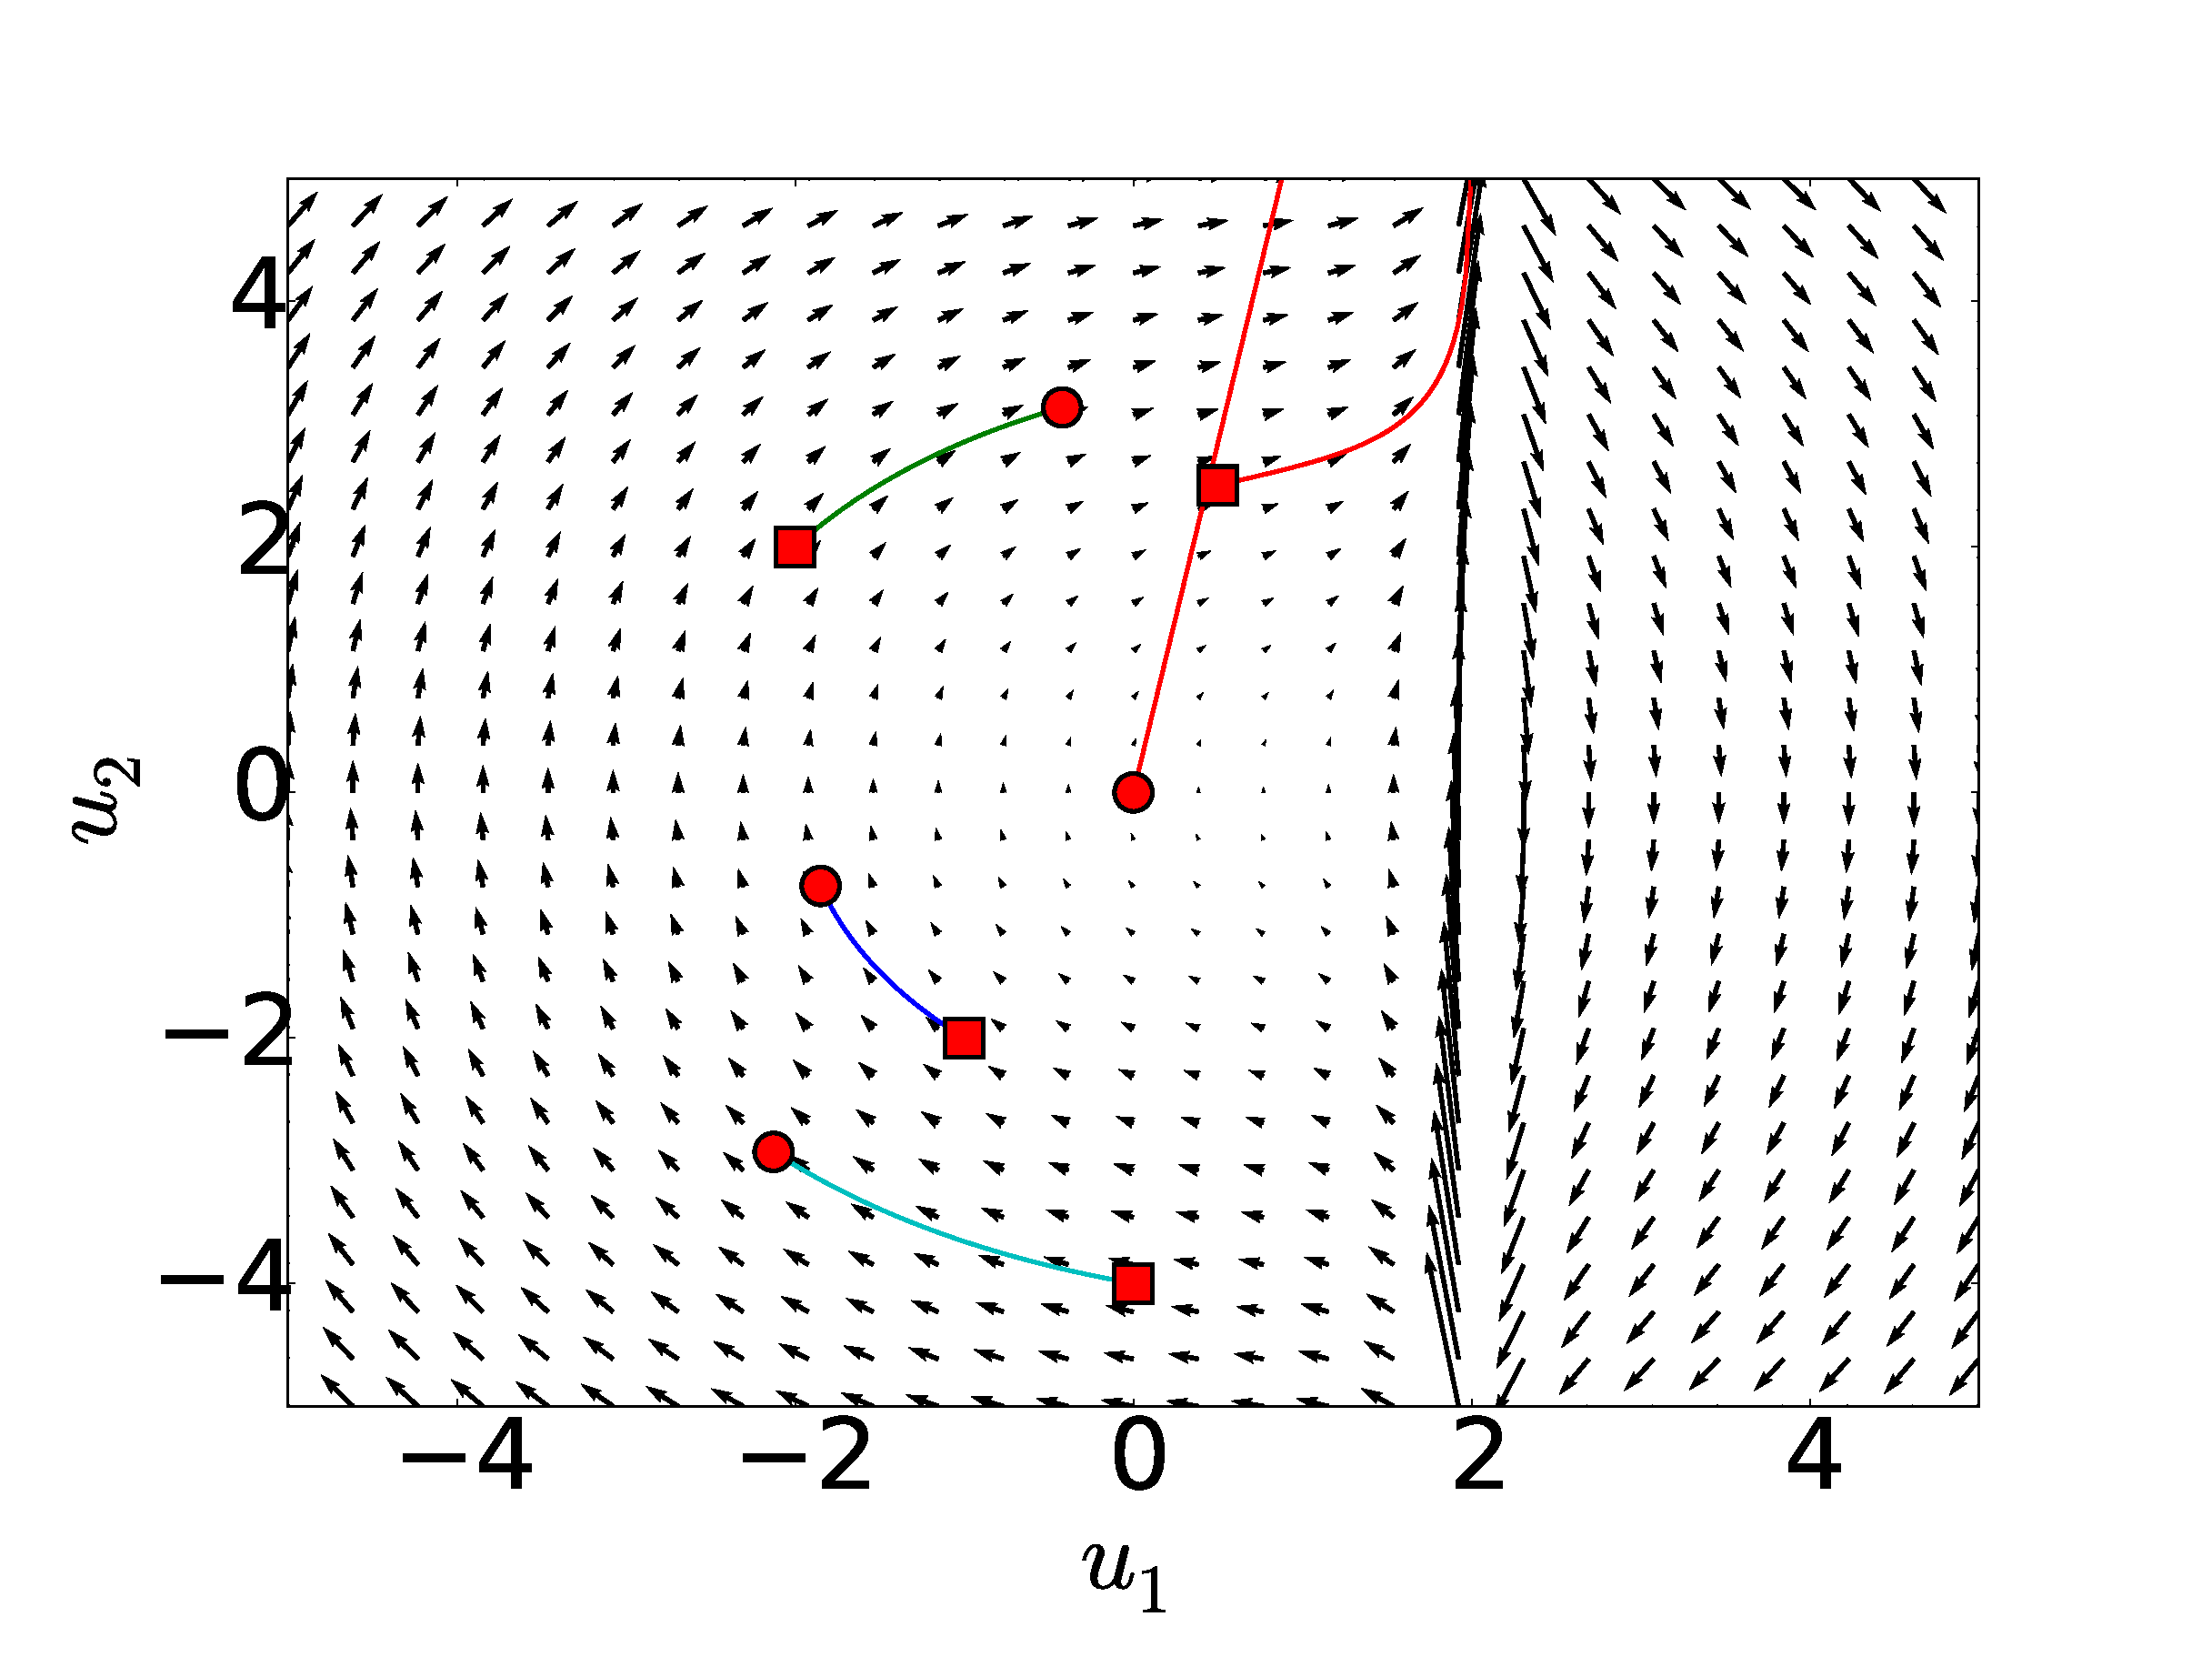
\includegraphics[width=8.0 cm]{figure/phase_a20_lambda20.eps}
		\caption{$a=2.0,\ \lambda = 2.0$}
    \end{subfigure}
    \caption{Phase plot and trajectories of the solution for different values of $a$, $\lambda$, and boundary conditions. $\Square$ represents the initial point and $\circ$ represents the final point of the trajectory.}
    \label{fig:phasePlot}
\end{figure}
%
% =================================================================
\newpage
{\flushleft\large{\textbf{2) Construct the phase portrate for the following differential equations}}}

The phase portrait is constructed by writing the equation of motion in the state-space and calculate the tangent vector to the solution at each point in the state-space at time zero. For all of the following equation we choose our states as follows
%
\begin{equation*}
\begin{aligned}
	x_1 &= x \\
	x_2 &= \dot{x}_1
\end{aligned}
\end{equation*}
%
After rewriting the equation is the state-space, we use Python's \texttt{numpy.meshgrid()} to generate a mesh over our state variables, $x_1$, $x_2$. By substituting these variables in our state equation, we can get the tangents to the solution at each point. These tangents are plotted using \texttt{matplotlib.pyplot.quiver} function in Python. A sample code is available in the appendix.

The following are the state-space representation of the second order differential equations for this problem.
%
\begin{align}
\ddot{x} + x + x^3 &= 0 \longrightarrow
\begin{bmatrix}
	\dot{x}_1 \\
	\dot{x}_2
\end{bmatrix} = 
\begin{bmatrix}
	x_2 \\
	-x_1 - x_1^3
\end{bmatrix} \\
% ---------------------------------- %
\ddot{x} + x - x^3 &= 0 \longrightarrow
\begin{bmatrix}
	\dot{x}_1 \\
	\dot{x}_2
\end{bmatrix} = 
\begin{bmatrix}
	x_2 \\
	-x_1 + x_1^3
\end{bmatrix} \\
% ---------------------------------- %
\ddot{x} - x + x^3 &= 0 \longrightarrow
\begin{bmatrix}
	\dot{x}_1 \\
	\dot{x}_2
\end{bmatrix} = 
\begin{bmatrix}
	x_2 \\
	x_1 - x_1^3
\end{bmatrix} \\
% ---------------------------------- %
\ddot{x} - x - x^3 &= 0 \longrightarrow
\begin{bmatrix}
	\dot{x}_1 \\
	\dot{x}_2
\end{bmatrix} = 
\begin{bmatrix}
	x_2 \\
	x_1 + x_1^3
\end{bmatrix} \\
% ---------------------------------- %
\ddot{x} + x^3 &= 0 \longrightarrow
\begin{bmatrix}
	\dot{x}_1 \\
	\dot{x}_2
\end{bmatrix} = 
\begin{bmatrix}
	x_2 \\
	x_1^3
\end{bmatrix}
\end{align}
%
The phase plots for these equations are shown in the Figure \ref{fig:phasePortrait}. The lines plotted on the phase plot represent the trajectory of the system with different initial conditions. The blue, cyan, and black lines have initial location of $0.5$, $1.5$, $2.0$ and initial velocity of $0.0$, $-1.0$, $1.5$ respectively. The square represents the origin of the trajectory and circle represents its end. 
%
\begin{figure}[H]
    \centering
    \begin{subfigure}[t]{7 cm}
        \centering
        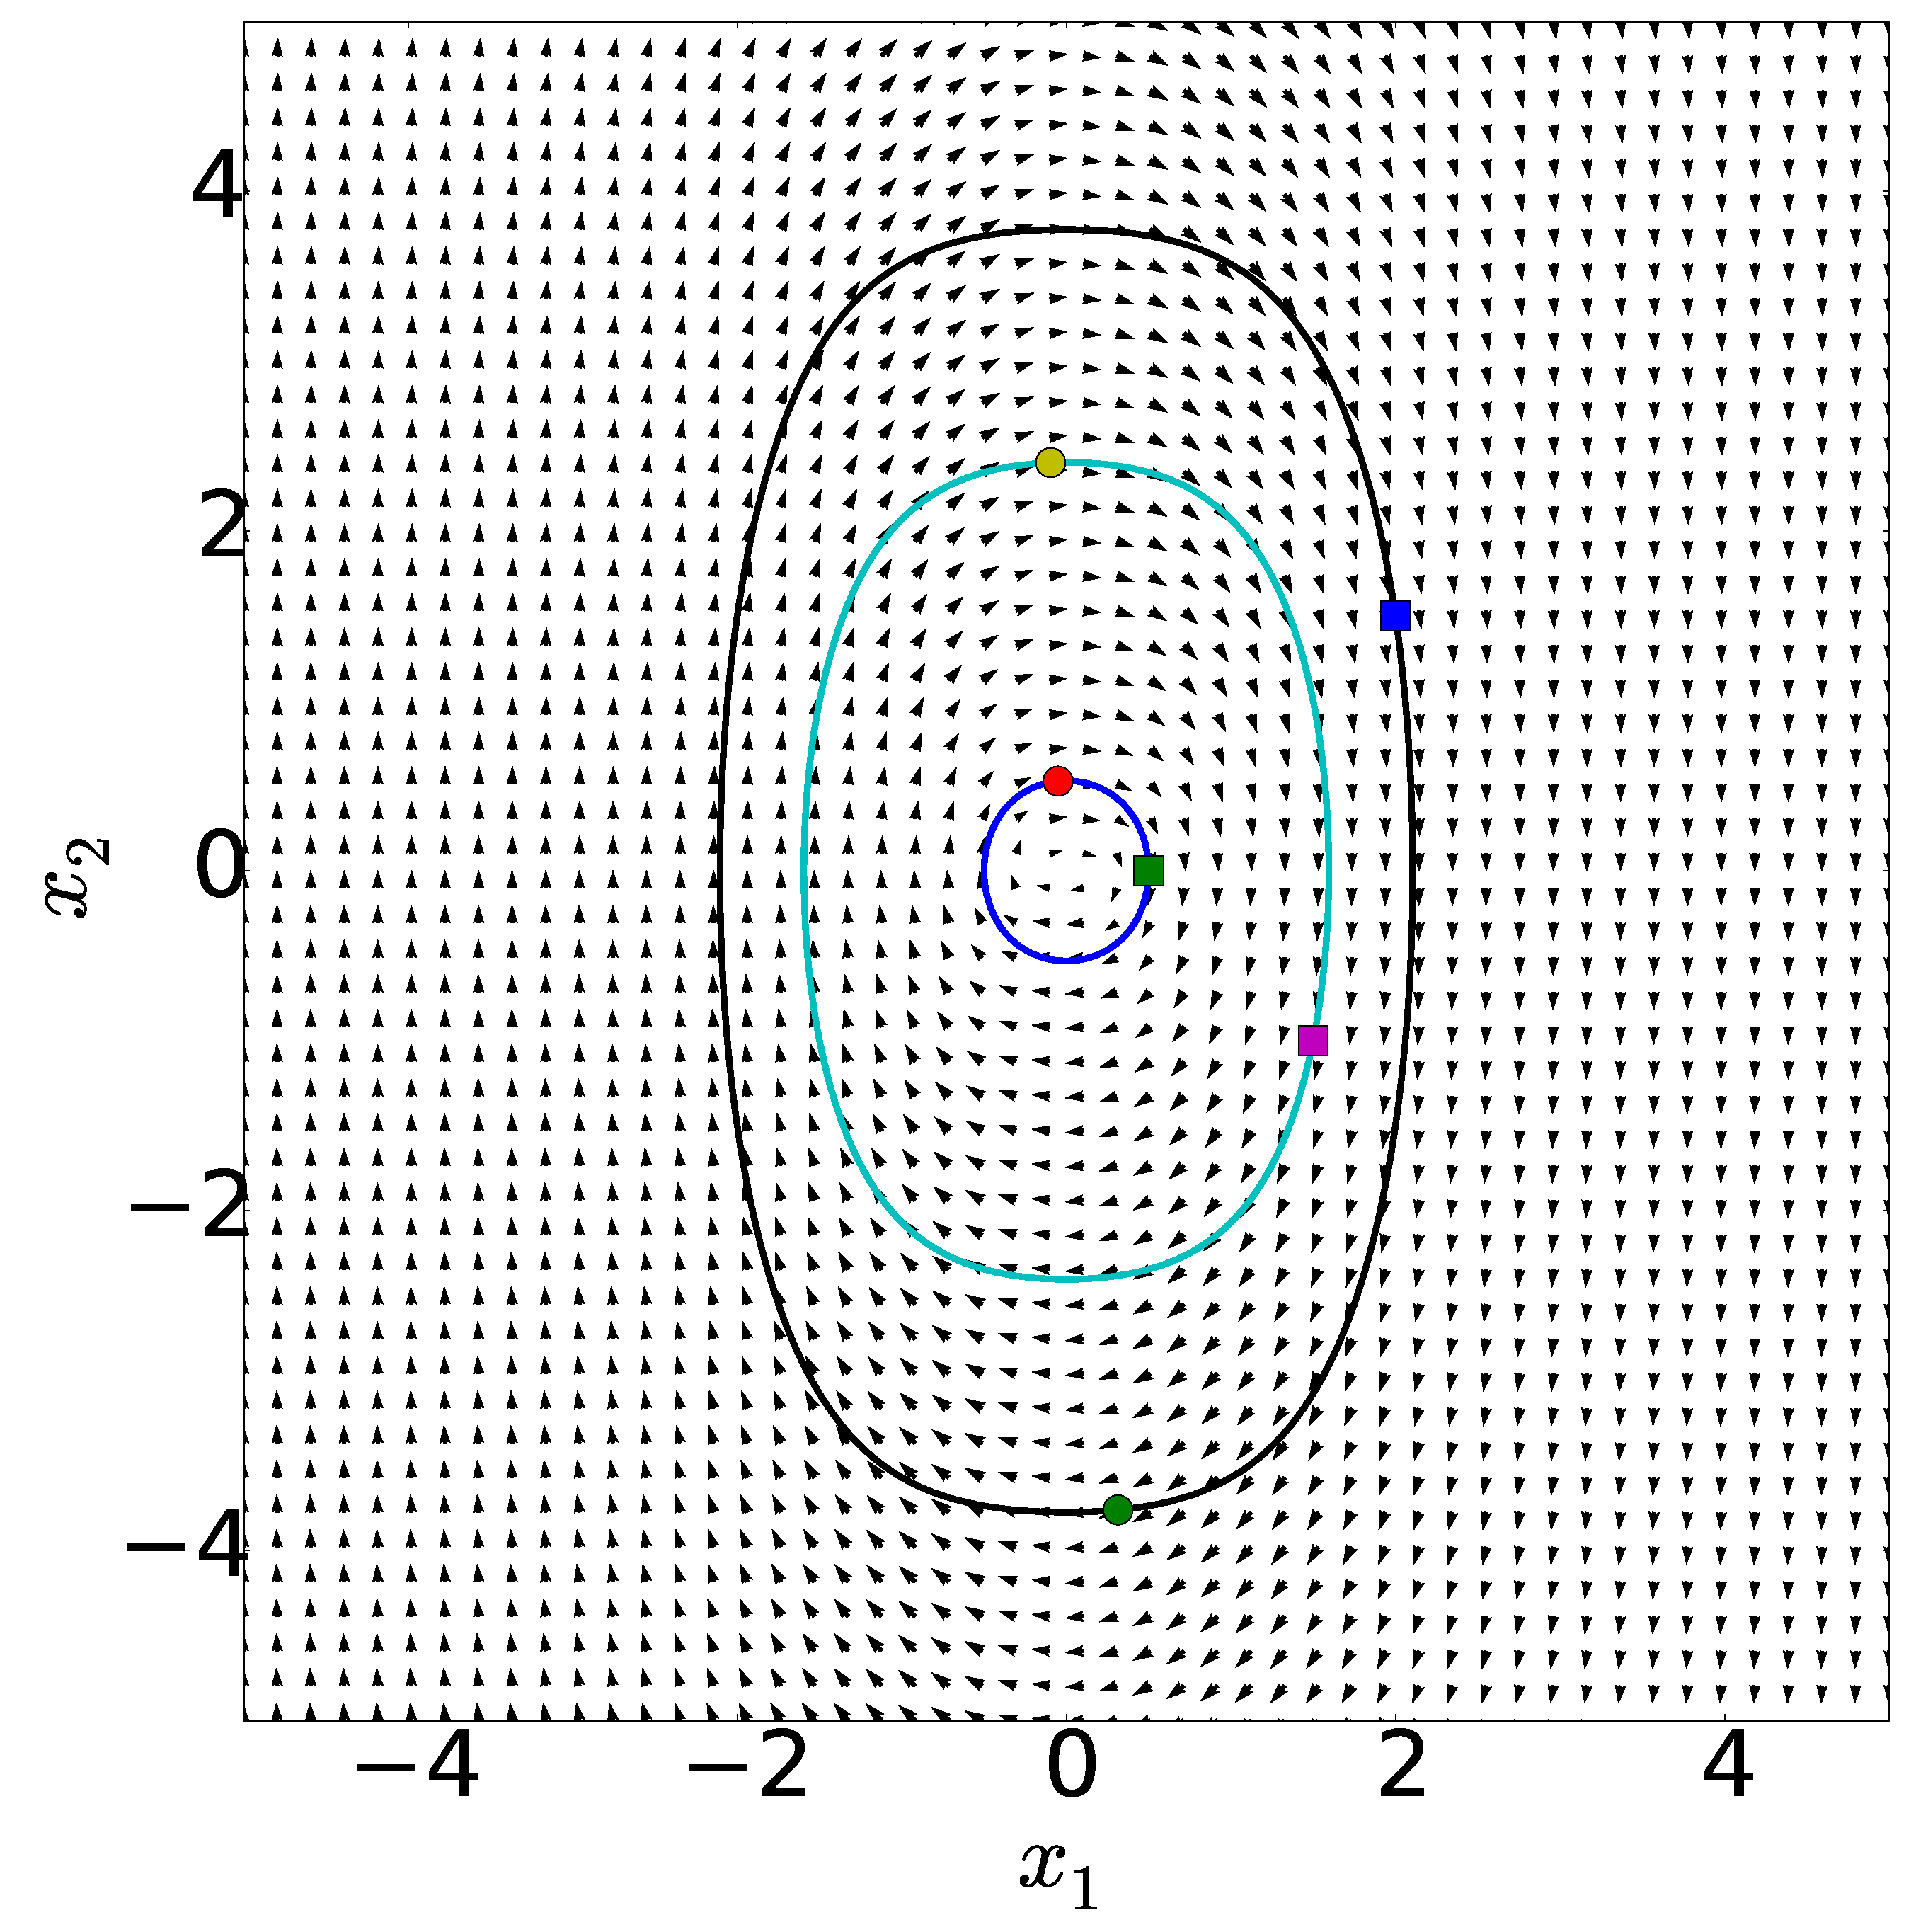
\includegraphics[height=7 cm]{figure/2A.eps}
        \caption{$\ddot{x} + x + x^3 = 0$}
    \end{subfigure}
    \quad
    \begin{subfigure}[t]{7 cm}
        \centering
        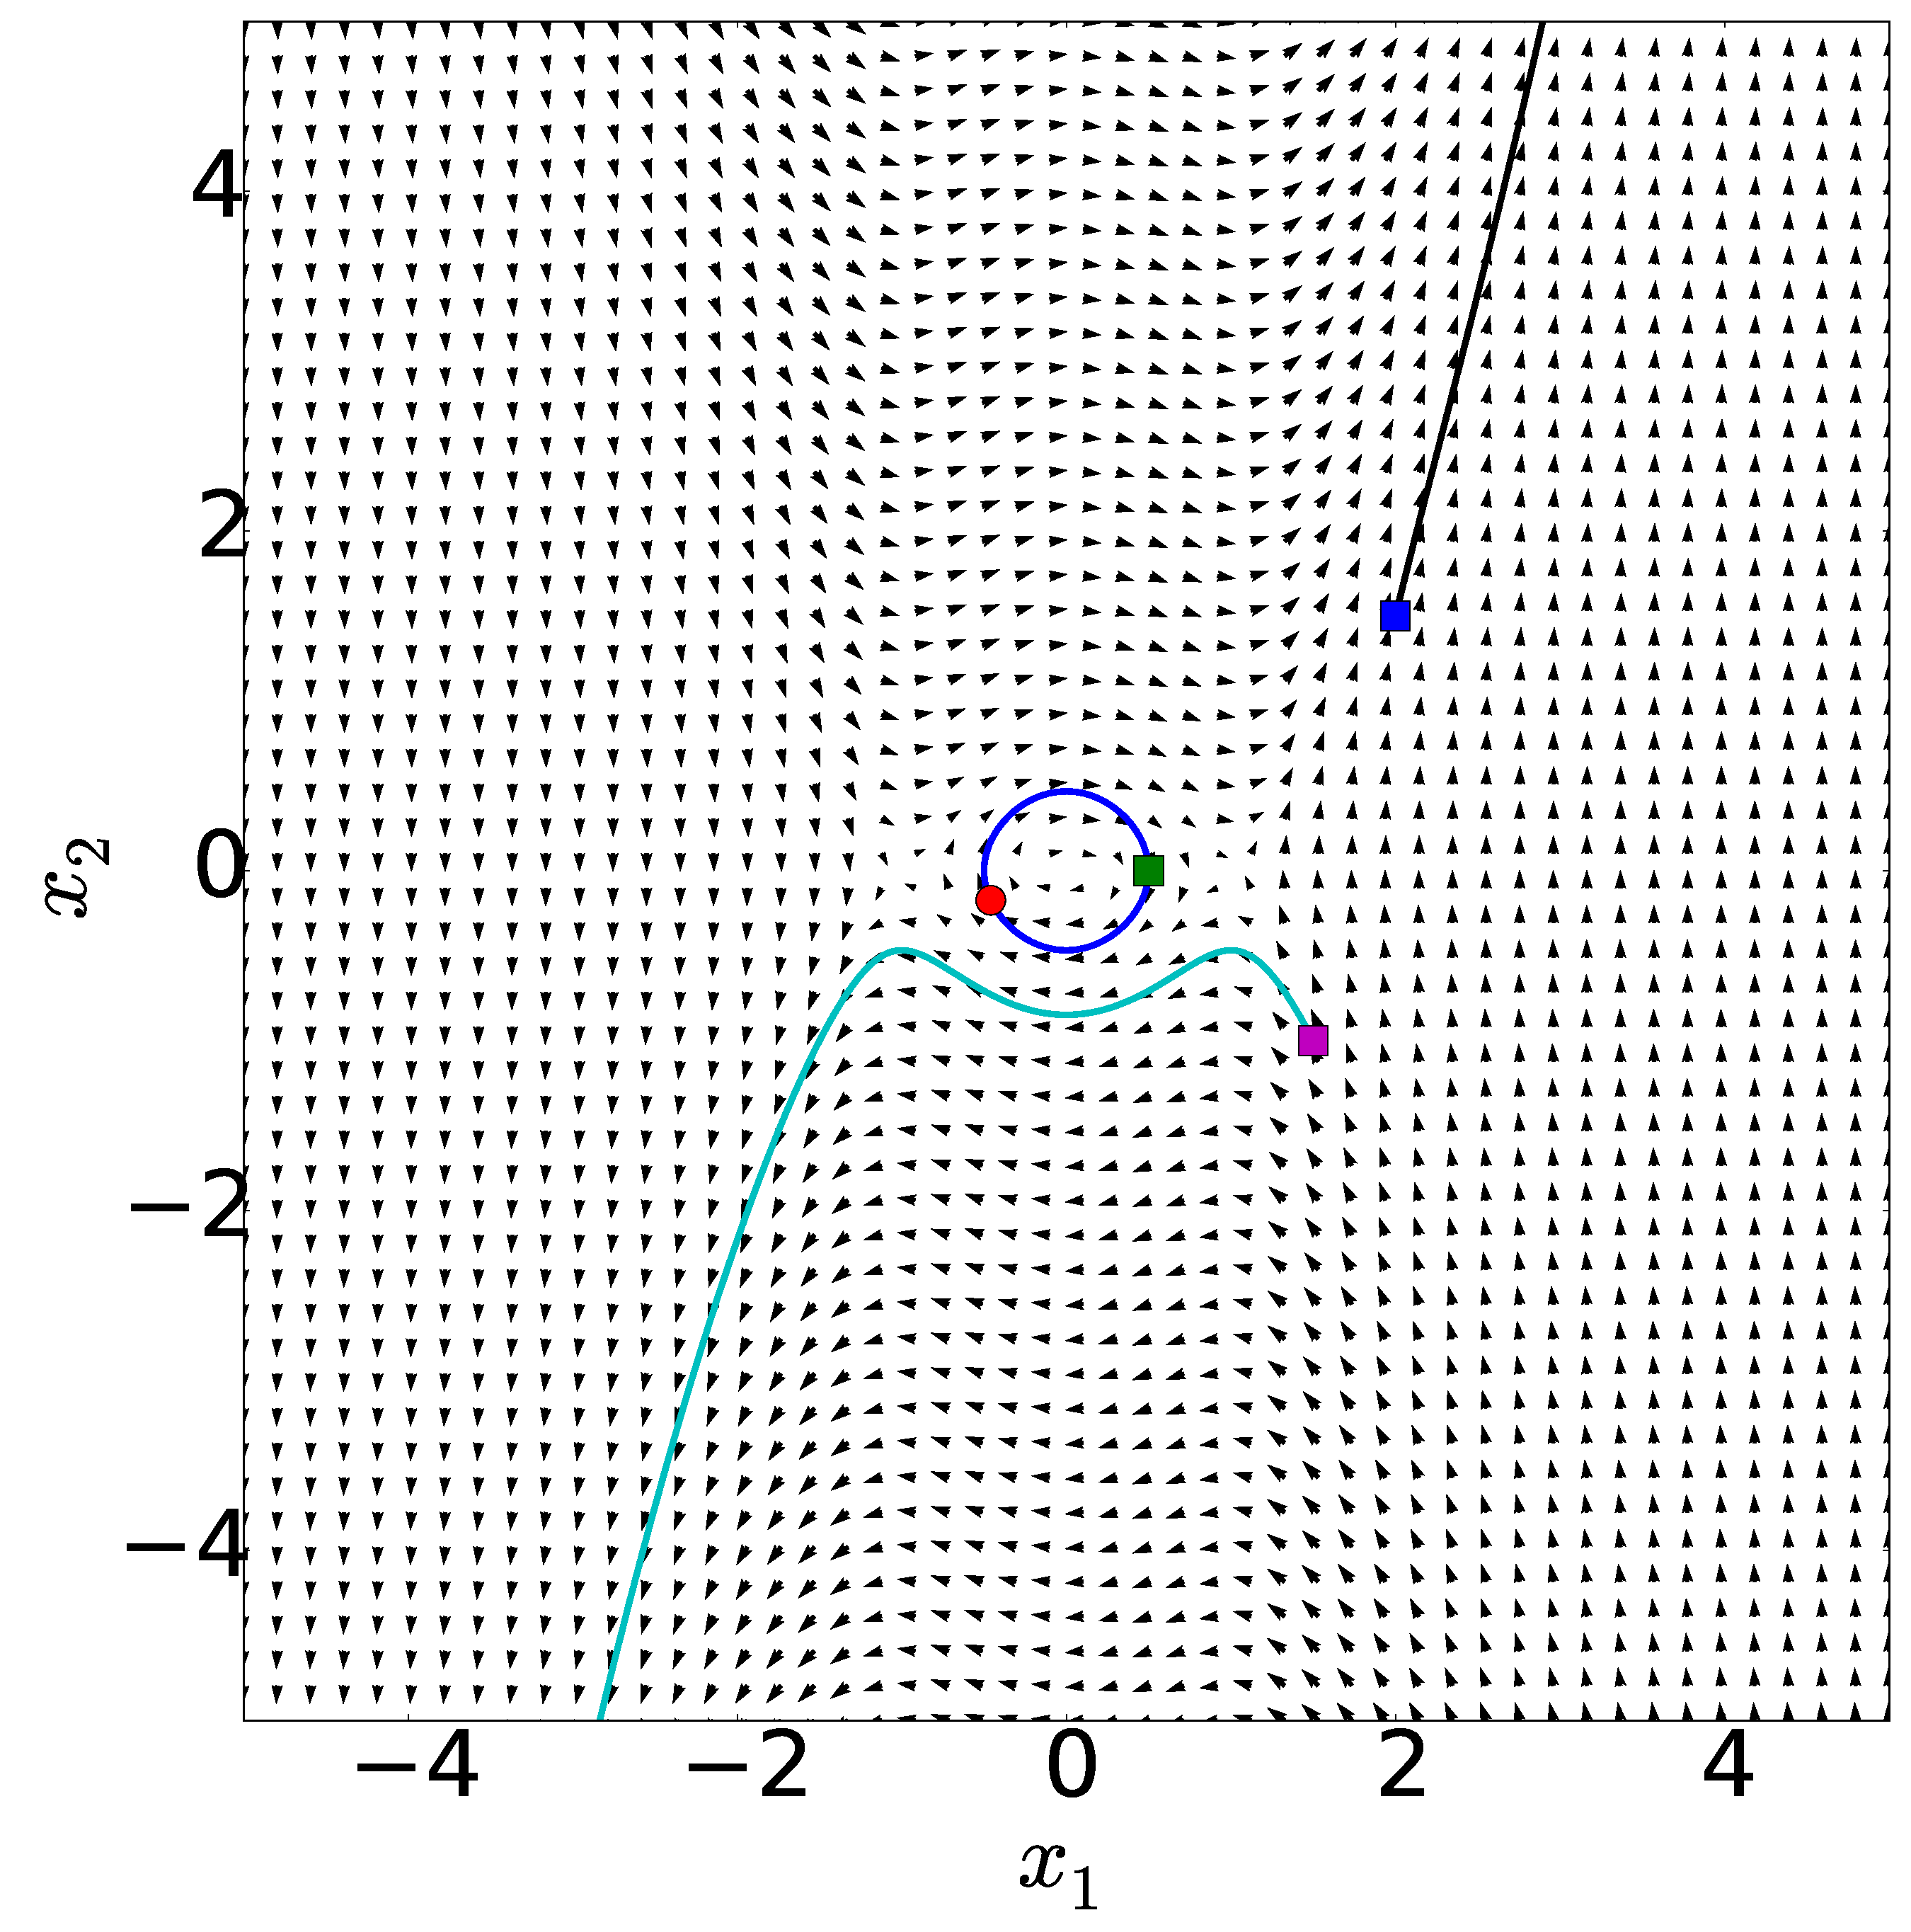
\includegraphics[height=7 cm]{figure/2B.eps}
        \caption{$\ddot{x} + x - x^3 = 0$}
    \end{subfigure}
    \\
    \begin{subfigure}[t]{7 cm}
        \centering
        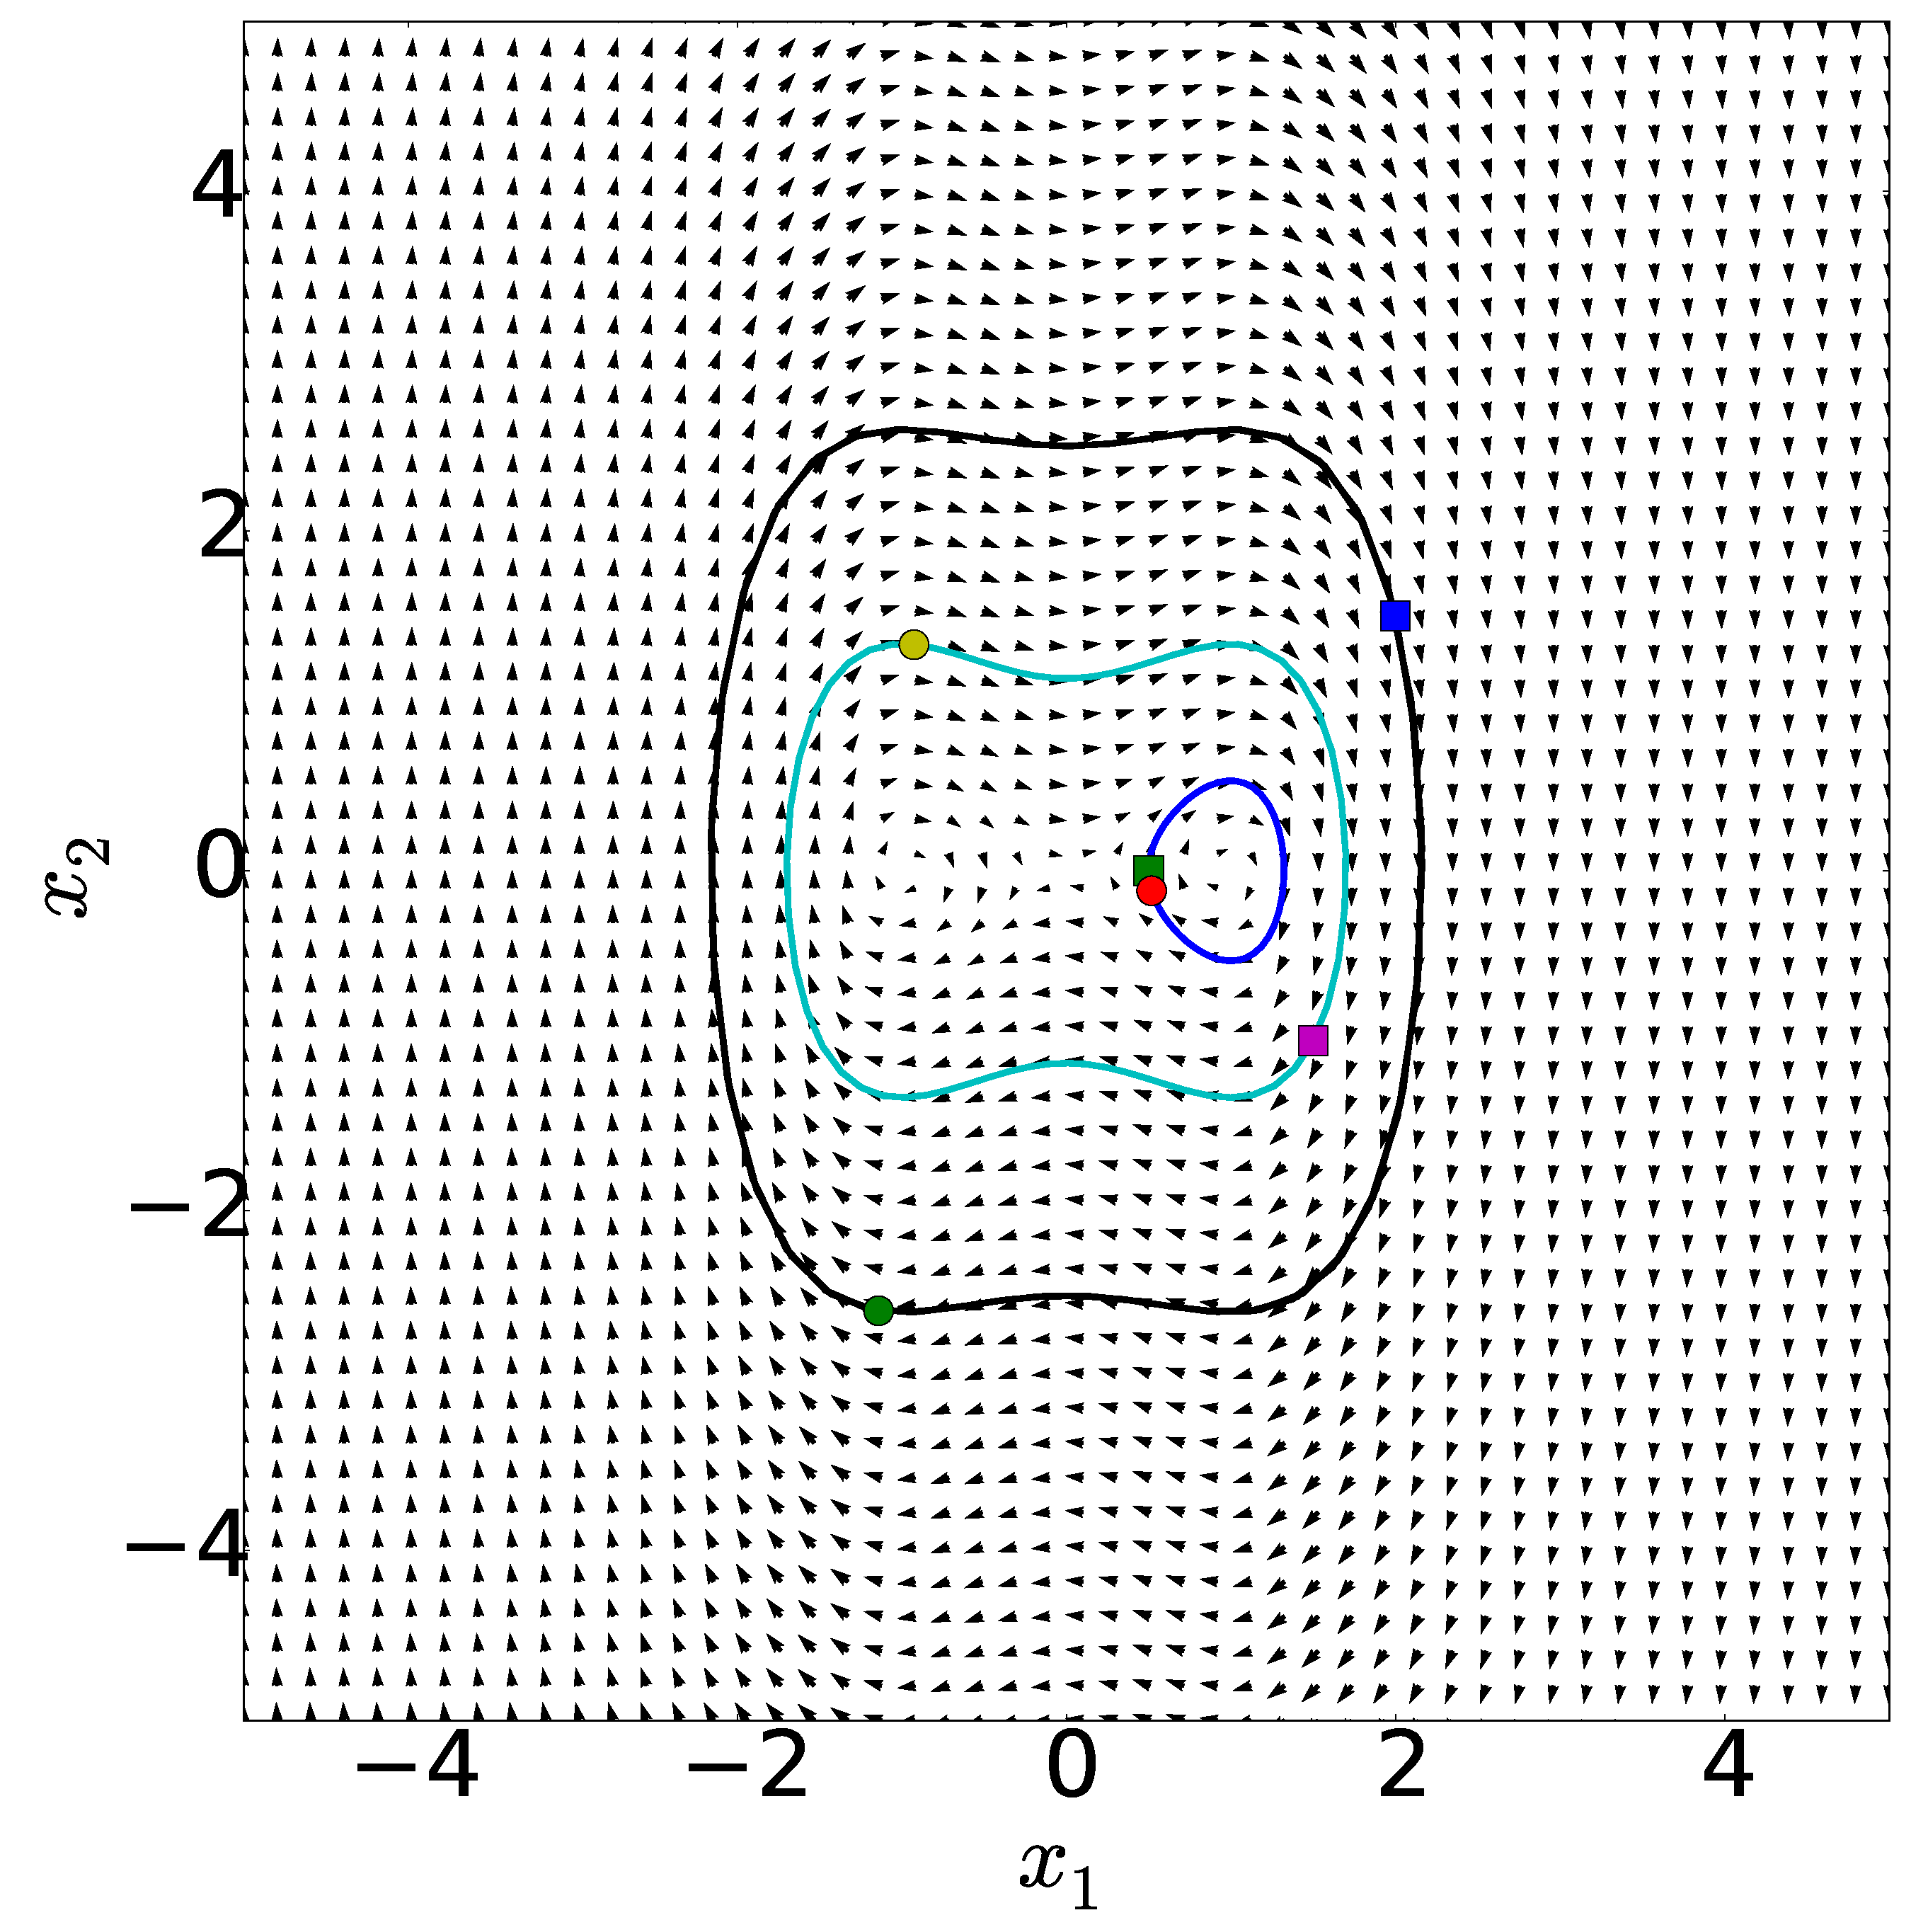
\includegraphics[height=7 cm]{figure/2C.eps}
        \caption{$\ddot{x} - x + x^3 = 0$}
    \end{subfigure}
    \quad
    \begin{subfigure}[t]{7 cm}
        \centering
        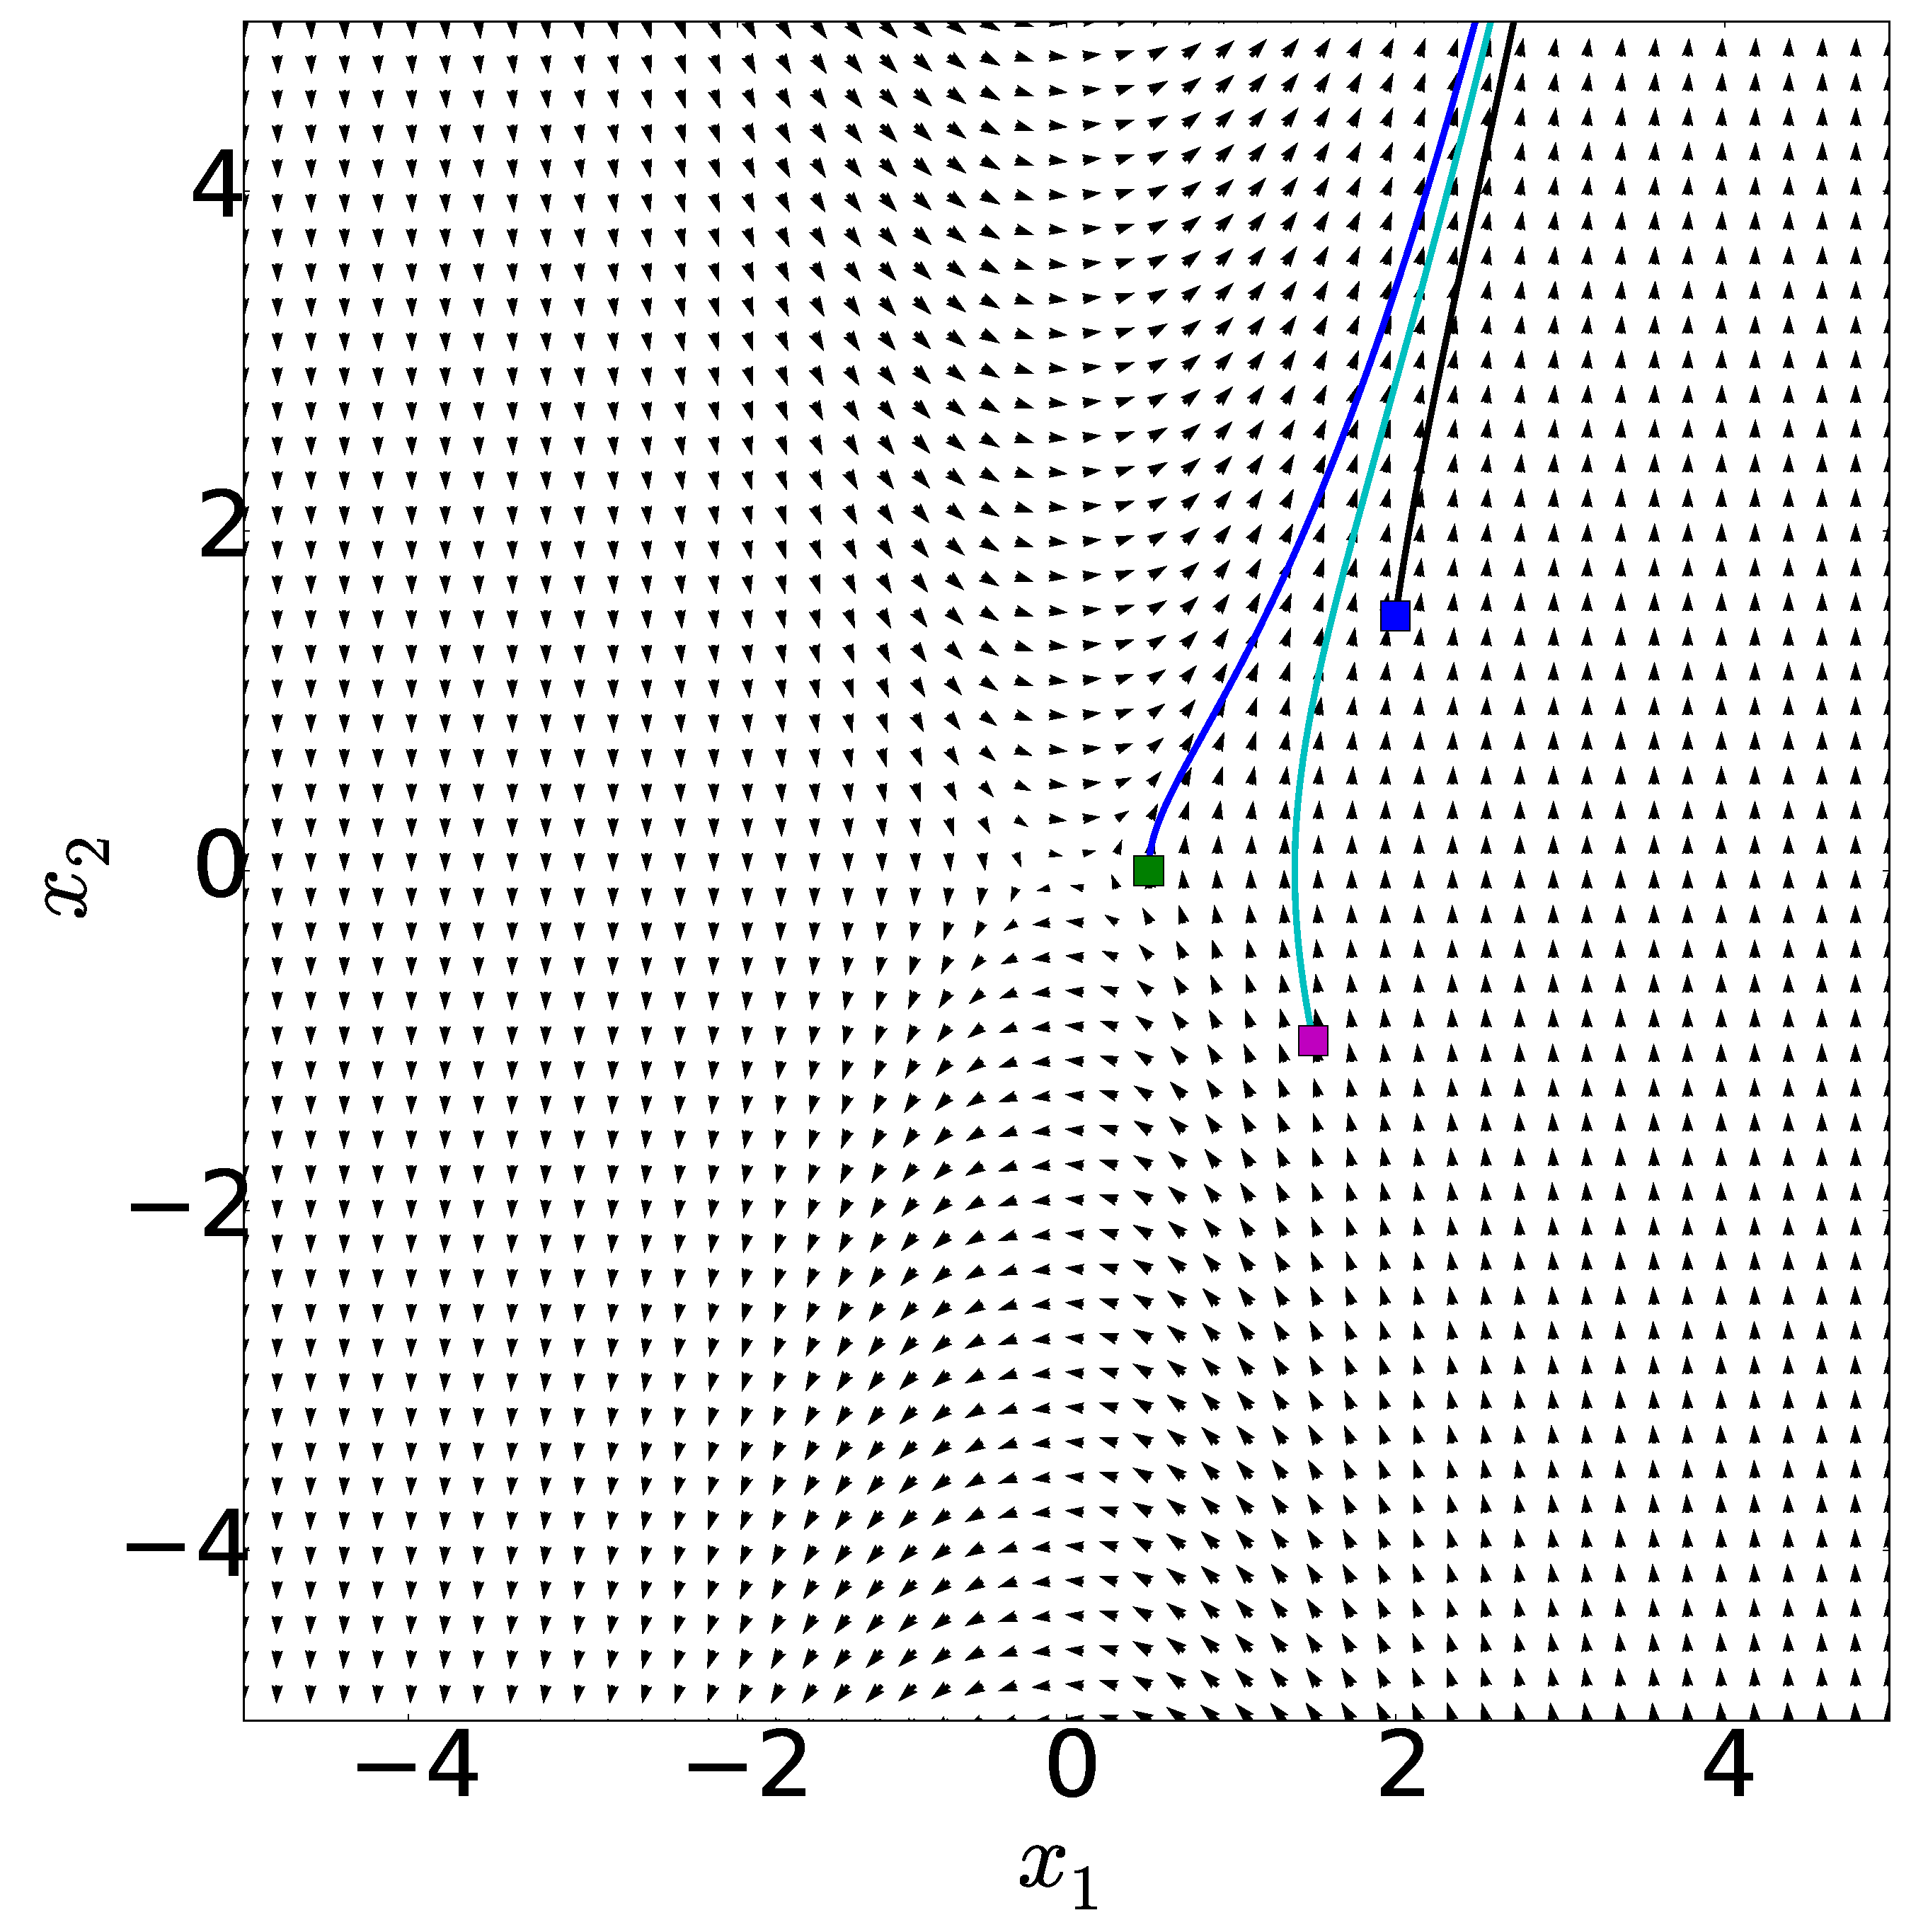
\includegraphics[height=7 cm]{figure/2D.eps}
        \caption{$\ddot{x} - x - x^3 = 0$}
    \end{subfigure}
    \\
    \begin{subfigure}[t]{7 cm}
        \centering
        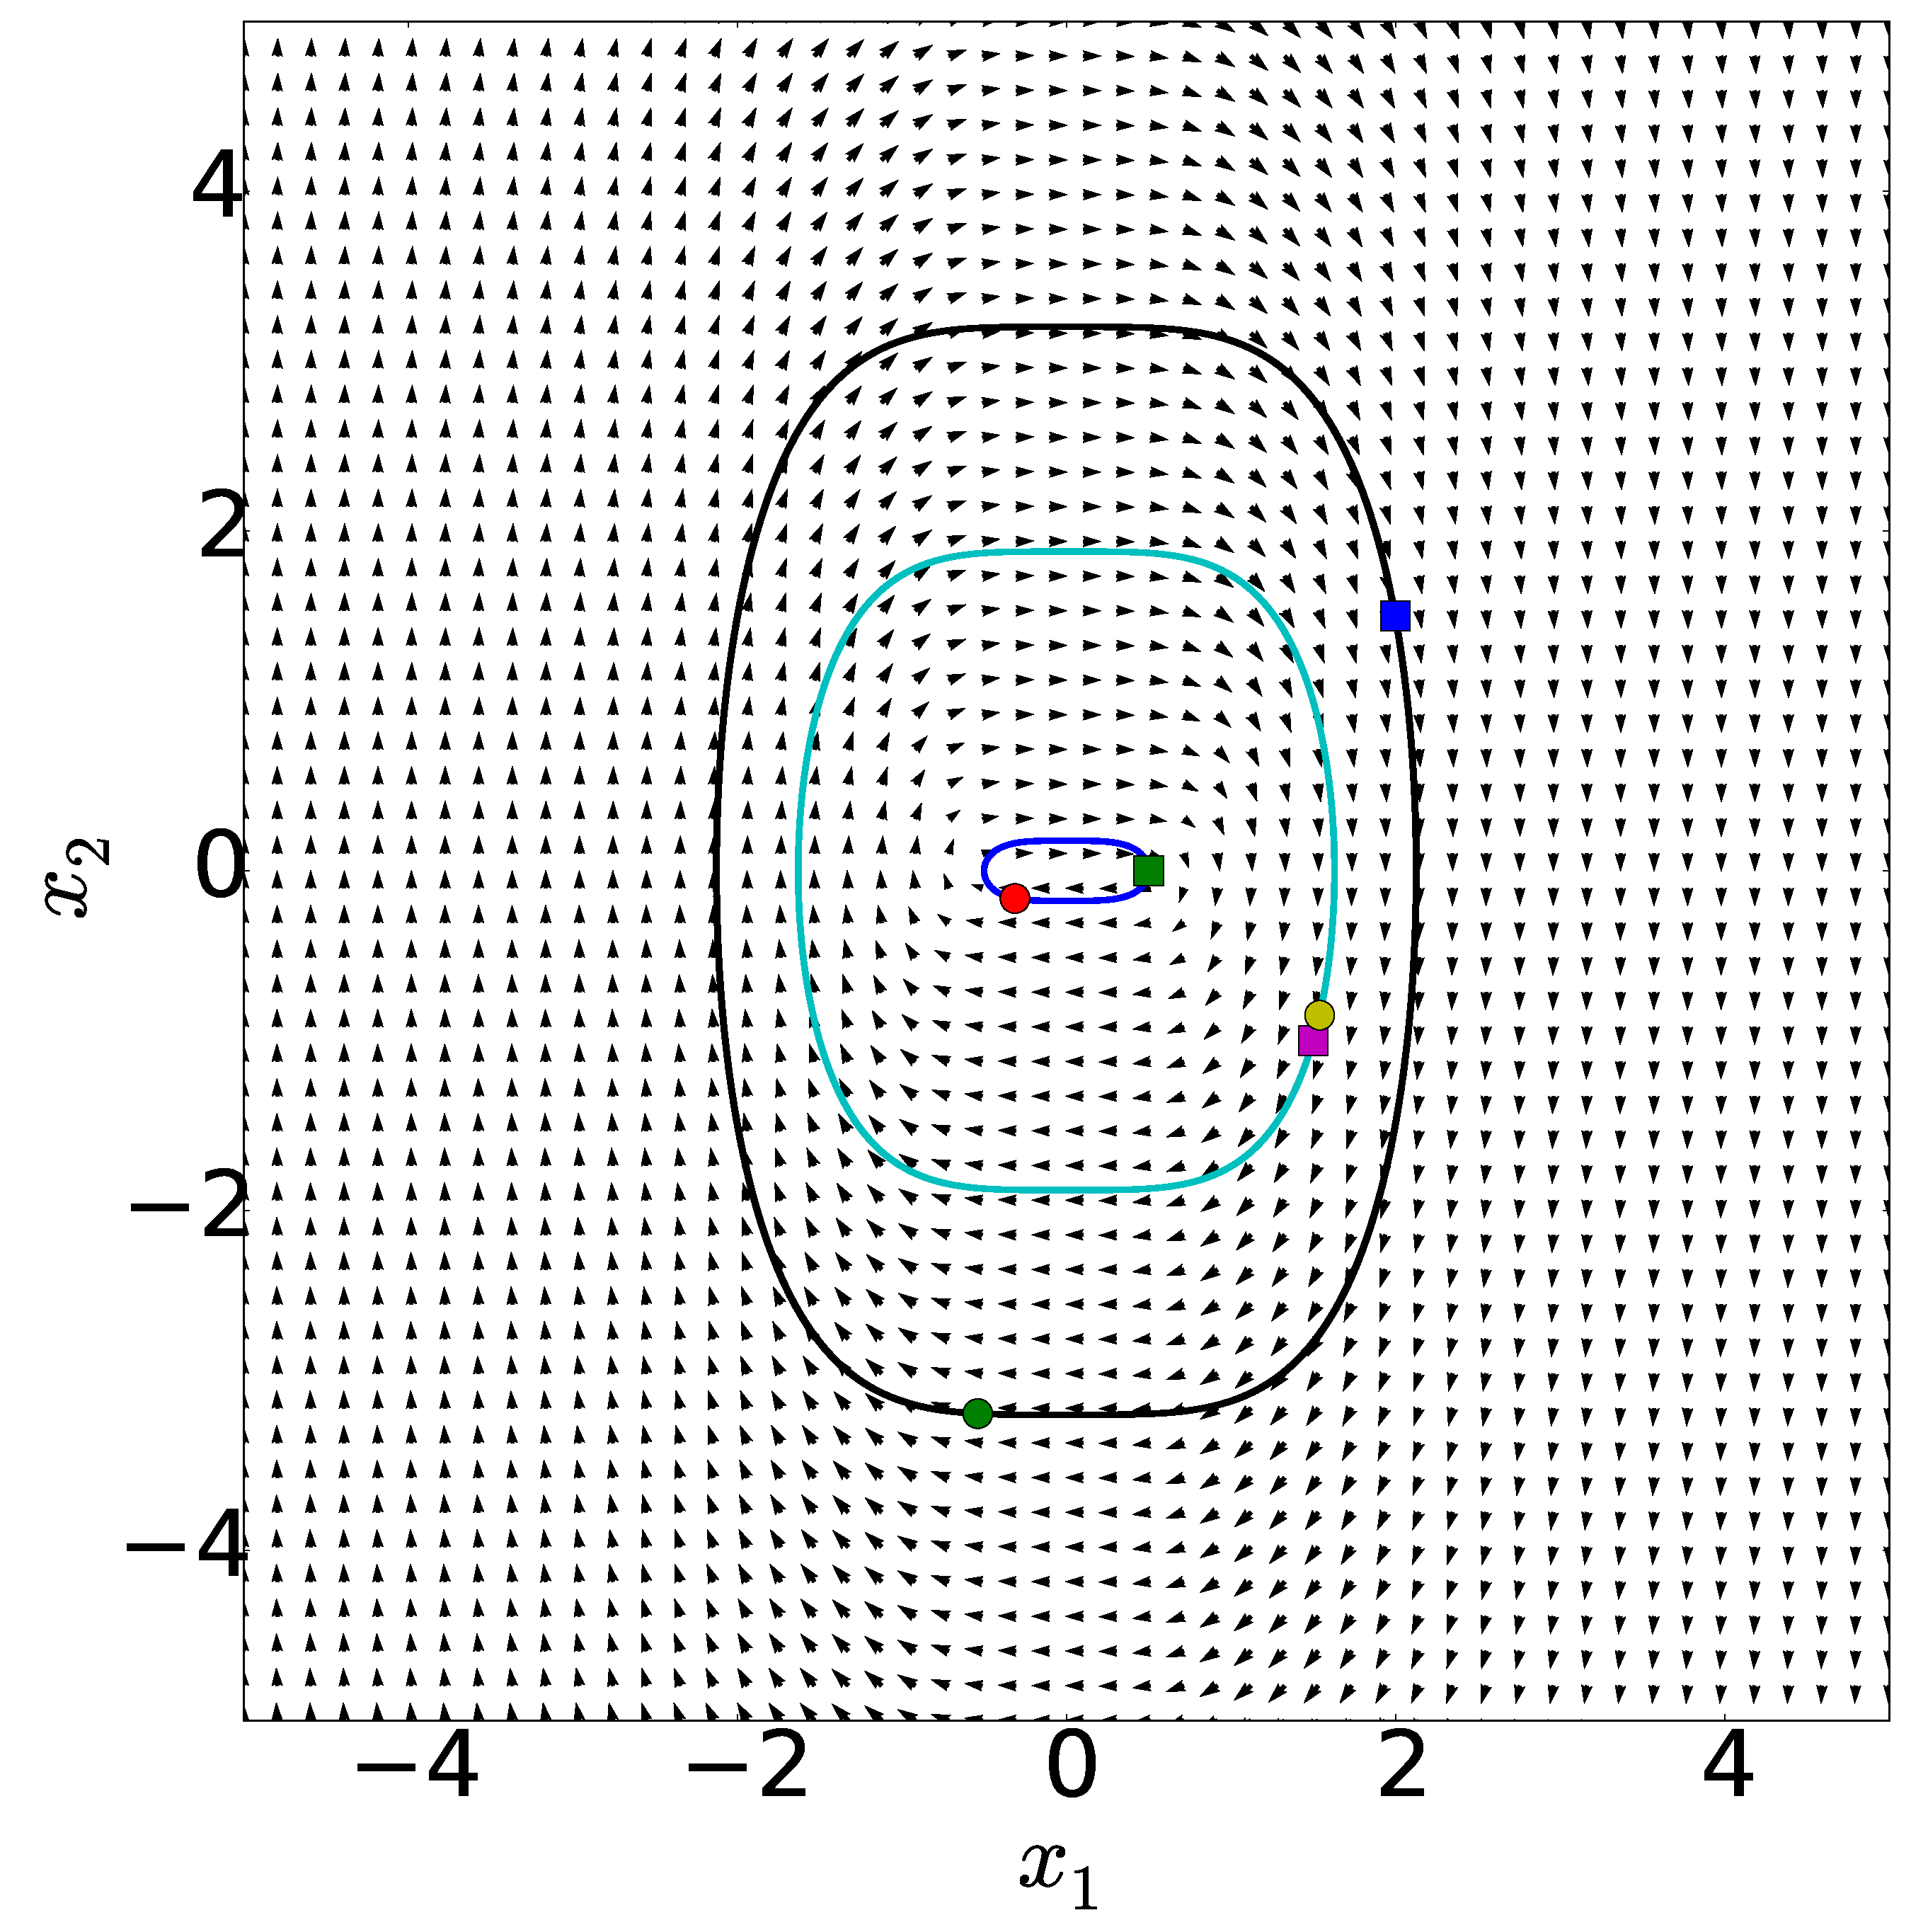
\includegraphics[height=7 cm]{figure/2E.eps}
        \caption{$\ddot{x} + x^3 = 0$}
    \end{subfigure}
    \caption{Phase portrait plot.}
    \label{fig:phasePortrait}
\end{figure}
%
As can be seen from the phase plots in Figure \ref{fig:phasePortrait}, Equations (1), (3), and (5) are stable system. It is also clear than Equations (1) and (5) have one equilibrium solution whereas (3) has two. Equation (2) is asymptotically stable. It has stable solution for initial conditions near the equilibrium point and becomes unstable when the the initial point moves further. Equation (4) is unstable as can be seen in Figure \ref{fig:phasePortrait}.
% ========================================================
\newpage
{\flushleft\large{\textbf{3) Determine when the following set of equations are dissipative and when the are conservative}}}
%
\begin{equation}
\begin{aligned}
	\dot{x} &= \sigma (y - x) \\
	\dot{y} &= \rho x - y - xz \\
	\dot{z} &= -\beta z + xy
\end{aligned}
\end{equation}
%
The divergence of above vector field can be written as follows:
%
\begin{equation}\label{eq:divergence3}
	\frac{\partial \dot{x}}{\partial x} +
	\frac{\partial \dot{y}}{\partial y} +
	\frac{\partial \dot{z}}{\partial z} = 
	-\sigma - 1 - \beta
\end{equation}
%
Depending on the sign of the Equation \eqref{eq:divergence3}, the system can be dissipative or conservative. If above equation is negative the system is dissipative, and if it is zero the system is conservative. This is can be written as follows:
%
\begin{equation}
\begin{cases}
	\sigma + \beta &= -1, \quad \text{conservative system} \\
	\sigma + \beta &< -1, \quad \text{disipative system}
\end{cases}
\end{equation}
%
$\rho$ is a free parameter for this problem.
% ========================================================
\newpage
{\flushleft\large{\textbf{4) Determine when the following set of equations are dissipative and when the are conservative}}}
%
\begin{equation}
\begin{aligned}
	\dot{x} &= -(y + z) \\
	\dot{y} &= x + ay \\
	\dot{z} &= b + (x - c)z
\end{aligned}
\end{equation}
%
The divergence of above vector field can be written as follows:
%
\begin{equation}\label{eq:divergence4}
	\frac{\partial \dot{x}}{\partial x} +
	\frac{\partial \dot{y}}{\partial y} +
	\frac{\partial \dot{z}}{\partial z} = 
	a + x - c
\end{equation}
%
Depending on the sign of the Equation \eqref{eq:divergence4}, the system can be dissipative or conservative. If above equation is negative the system is dissipative, and if it is zero the system is conservative. This is can be written as follows:
%
\begin{equation}
\begin{cases}
	c - a = x, \quad &\text{conservative system} \\
	c - a > x, \quad &\text{disipative system}
\end{cases}
\end{equation}
%
$b$ is the free parameters for this problem.
% ========================================================
\newpage
{\flushleft\large{\textbf{5) Determine when the following map is dissipative}}}
%
\begin{equation}\label{eq:5}
\begin{aligned}
	x_{n+1} = a_{11} x_n + a_{12}y_n \\
	y_{n+1} = a_{21} x_n + a_{22}y_n
\end{aligned}
\end{equation}
%
A map is said to be dissipative at $\mathbf{x}_k = \mathbf{x}_0$ if
%
\begin{equation}
	|\det D_{\mathbf{x}_k} \mathbf{F}| < 1 \quad \text{at} \quad \mathbf{x}_k = \mathbf{x}_0
\end{equation}
%
For Equation \eqref{eq:5} we have
%
\begin{equation}
|\det D_{\mathbf{x}_k} \mathbf{F}| = 
\left|
\begin{bmatrix}
a_{11} &a_{12} \\
a_{21} &a_{22}
\end{bmatrix}
\right| = 
a_{11} \times a_{22} - a_{12} \times a_{21}
\end{equation}
%
For the system to be dissipative we should have
%
\begin{equation}
	a_{11} \times a_{22} - a_{12} \times a_{21} < 0
\end{equation}
% 
% ========================================================
\newpage
\center\large{\textbf{Appendix}}
\lstinputlisting{code/sample_code.py}
\end{document}